\documentclass{book}
\usepackage{amsmath}
\usepackage{xcolor}
\usepackage{hyperref}
\usepackage{titling}
\usepackage{multirow}
\usepackage{setspace}
\usepackage{makeidx}
\usepackage{tikz}
\usepackage{subfigure}
\usepackage{braket}
\usepackage{graphicx}
\usepackage{qcircuit}
\usepackage{array}
\usepackage{tabularray}
\usepackage{circuitikz}
\usepackage{amssymb}
\usepackage{setspace}
\usepackage{pgfpages}
\usepackage{color}
\usepackage{fancyvrb}
\usepackage{tcolorbox}



\linespread{1.5}

% ---------------


% Options for packages loaded elsewhere
\PassOptionsToPackage{unicode}{hyperref}
\PassOptionsToPackage{hyphens}{url}
%

\usepackage{amsmath,amssymb}
\usepackage{lmodern}
\usepackage{iftex}
\ifPDFTeX
\usepackage[T1]{fontenc}
\usepackage[utf8]{inputenc}
\usepackage{textcomp} % provide euro and other symbols
\else % if luatex or xetex
\usepackage{unicode-math}
\defaultfontfeatures{Scale=MatchLowercase}
\defaultfontfeatures[\rmfamily]{Ligatures=TeX,Scale=1}
\fi
% Use upquote if available, for straight quotes in verbatim environments
\IfFileExists{upquote.sty}{\usepackage{upquote}}{}
\IfFileExists{microtype.sty}{% use microtype if available
	\usepackage[]{microtype}
	\UseMicrotypeSet[protrusion]{basicmath} % disable protrusion for tt fonts
}{}
\makeatletter
\@ifundefined{KOMAClassName}{% if non-KOMA class
	\IfFileExists{parskip.sty}{%
		\usepackage{parskip}
	}{% else
		\setlength{\parindent}{0pt}
		\setlength{\parskip}{6pt plus 2pt minus 1pt}}
}{% if KOMA class
	\KOMAoptions{parskip=half}}
\makeatother
\IfFileExists{xurl.sty}{\usepackage{xurl}}{} % add URL line breaks if available
\IfFileExists{bookmark.sty}{\usepackage{bookmark}}{\usepackage{hyperref}}
\hypersetup{
	hidelinks,
	pdfcreator={LaTeX via pandoc}}
\urlstyle{same} % disable monospaced font for URLs

\newcommand{\VerbBar}{|}
\newcommand{\VERB}{\Verb[commandchars=\\\{\}]}
\DefineVerbatimEnvironment{Highlighting}{Verbatim}{commandchars=\\\{\}}
% Add ',fontsize=\small' for more characters per line
\newenvironment{Shaded}{}{}
\newcommand{\AlertTok}[1]{\textcolor[rgb]{1.00,0.00,0.00}{\textbf{#1}}}
\newcommand{\AnnotationTok}[1]{\textcolor[rgb]{0.38,0.63,0.69}{\textbf{\textit{#1}}}}
\newcommand{\AttributeTok}[1]{\textcolor[rgb]{0.49,0.56,0.16}{#1}}
\newcommand{\BaseNTok}[1]{\textcolor[rgb]{0.25,0.63,0.44}{#1}}
\newcommand{\BuiltInTok}[1]{#1}
\newcommand{\CharTok}[1]{\textcolor[rgb]{0.25,0.44,0.63}{#1}}
\newcommand{\CommentTok}[1]{\textcolor[rgb]{0.38,0.63,0.69}{\textit{#1}}}
\newcommand{\CommentVarTok}[1]{\textcolor[rgb]{0.38,0.63,0.69}{\textbf{\textit{#1}}}}
\newcommand{\ConstantTok}[1]{\textcolor[rgb]{0.53,0.00,0.00}{#1}}
\newcommand{\ControlFlowTok}[1]{\textcolor[rgb]{0.00,0.44,0.13}{\textbf{#1}}}
\newcommand{\DataTypeTok}[1]{\textcolor[rgb]{0.56,0.13,0.00}{#1}}
\newcommand{\DecValTok}[1]{\textcolor[rgb]{0.25,0.63,0.44}{#1}}
\newcommand{\DocumentationTok}[1]{\textcolor[rgb]{0.73,0.13,0.13}{\textit{#1}}}
\newcommand{\ErrorTok}[1]{\textcolor[rgb]{1.00,0.00,0.00}{\textbf{#1}}}
\newcommand{\ExtensionTok}[1]{#1}
\newcommand{\FloatTok}[1]{\textcolor[rgb]{0.25,0.63,0.44}{#1}}
\newcommand{\FunctionTok}[1]{\textcolor[rgb]{0.02,0.16,0.49}{#1}}
\newcommand{\ImportTok}[1]{#1}
\newcommand{\InformationTok}[1]{\textcolor[rgb]{0.38,0.63,0.69}{\textbf{\textit{#1}}}}
\newcommand{\KeywordTok}[1]{\textcolor[rgb]{0.00,0.44,0.13}{\textbf{#1}}}
\newcommand{\NormalTok}[1]{#1}
\newcommand{\OperatorTok}[1]{\textcolor[rgb]{0.40,0.40,0.40}{#1}}
\newcommand{\OtherTok}[1]{\textcolor[rgb]{0.00,0.44,0.13}{#1}}
\newcommand{\PreprocessorTok}[1]{\textcolor[rgb]{0.74,0.48,0.00}{#1}}
\newcommand{\RegionMarkerTok}[1]{#1}
\newcommand{\SpecialCharTok}[1]{\textcolor[rgb]{0.25,0.44,0.63}{#1}}
\newcommand{\SpecialStringTok}[1]{\textcolor[rgb]{0.73,0.40,0.53}{#1}}
\newcommand{\StringTok}[1]{\textcolor[rgb]{0.25,0.44,0.63}{#1}}
\newcommand{\VariableTok}[1]{\textcolor[rgb]{0.10,0.09,0.49}{#1}}
\newcommand{\VerbatimStringTok}[1]{\textcolor[rgb]{0.25,0.44,0.63}{#1}}
\newcommand{\WarningTok}[1]{\textcolor[rgb]{0.38,0.63,0.69}{\textbf{\textit{#1}}}}
\setlength{\emergencystretch}{3em} % prevent overfull lines
\providecommand{\tightlist}{%
	\setlength{\itemsep}{0pt}\setlength{\parskip}{0pt}}
\setcounter{secnumdepth}{-\maxdimen} % remove section numbering
\ifLuaTeX
\usepackage{selnolig}  % disable illegal ligatures
\fi


\pgfpagesdeclarelayout{boxed}
{
	\edef\pgfpageoptionborder{0pt}
}
{
	\pgfpagesphysicalpageoptions
	{%
		logical pages=1,%
	}
	\pgfpageslogicalpageoptions{1}
	{
		border code=\pgfsetlinewidth{2pt}\pgfstroke,%
		border shrink=\pgfpageoptionborder,%
		resized width=.95\pgfphysicalwidth,%
		resized height=.95\pgfphysicalheight,%
		center=\pgfpoint{.5\pgfphysicalwidth}{.5\pgfphysicalheight}%
	}%
}



\pgfpagesuselayout{boxed}
\usepackage{url}
\usepackage{authblk}
\usepackage{amsmath}
\usepackage{setspace}\doublespacing
\usepackage{graphicx} 
\usepackage{amssymb}


\usepackage{amsfonts}
\usepackage{amssymb}
\usepackage{floatflt}
\usepackage{lipsum}
%\usepackage[demo]{graphicx}
\usepackage{upquote} % Upright quotes for verbatim code
\usepackage{eurosym} % defines \euro
\usepackage[mathletters]{ucs} % Extended unicode (utf-8) support
\usepackage[utf8x]{inputenc} % Allow utf-8 characters in the tex document

\usepackage{grffile} % extends the file name processing of package graphics 
\usepackage{xepersian}

\DefineVerbatimEnvironment{Highlighting}{Verbatim}{commandchars=\\\{\}}
% Pygments definitions

\makeatletter
\def\PY@reset{\let\PY@it=\relax \let\PY@bf=\relax%
	\let\PY@ul=\relax \let\PY@tc=\relax%
	\let\PY@bc=\relax \let\PY@ff=\relax}
\def\PY@tok#1{\csname PY@tok@#1\endcsname}
\def\PY@toks#1+{\ifx\relax#1\empty\else%
	\PY@tok{#1}\expandafter\PY@toks\fi}
\def\PY@do#1{\PY@bc{\PY@tc{\PY@ul{%
				\PY@it{\PY@bf{\PY@ff{#1}}}}}}}
\def\PY#1#2{\PY@reset\PY@toks#1+\relax+\PY@do{#2}}

\expandafter\def\csname PY@tok@w\endcsname{\def\PY@tc##1{\textcolor[rgb]{0.73,0.73,0.73}{##1}}}
\expandafter\def\csname PY@tok@c\endcsname{\let\PY@it=\textit\def\PY@tc##1{\textcolor[rgb]{0.25,0.50,0.50}{##1}}}
\expandafter\def\csname PY@tok@cp\endcsname{\def\PY@tc##1{\textcolor[rgb]{0.74,0.48,0.00}{##1}}}
\expandafter\def\csname PY@tok@k\endcsname{\let\PY@bf=\textbf\def\PY@tc##1{\textcolor[rgb]{0.00,0.50,0.00}{##1}}}
\expandafter\def\csname PY@tok@kp\endcsname{\def\PY@tc##1{\textcolor[rgb]{0.00,0.50,0.00}{##1}}}
\expandafter\def\csname PY@tok@kt\endcsname{\def\PY@tc##1{\textcolor[rgb]{0.69,0.00,0.25}{##1}}}
\expandafter\def\csname PY@tok@o\endcsname{\def\PY@tc##1{\textcolor[rgb]{0.40,0.40,0.40}{##1}}}
\expandafter\def\csname PY@tok@ow\endcsname{\let\PY@bf=\textbf\def\PY@tc##1{\textcolor[rgb]{0.67,0.13,1.00}{##1}}}
\expandafter\def\csname PY@tok@nb\endcsname{\def\PY@tc##1{\textcolor[rgb]{0.00,0.50,0.00}{##1}}}
\expandafter\def\csname PY@tok@nf\endcsname{\def\PY@tc##1{\textcolor[rgb]{0.00,0.00,1.00}{##1}}}
\expandafter\def\csname PY@tok@nc\endcsname{\let\PY@bf=\textbf\def\PY@tc##1{\textcolor[rgb]{0.00,0.00,1.00}{##1}}}
\expandafter\def\csname PY@tok@nn\endcsname{\let\PY@bf=\textbf\def\PY@tc##1{\textcolor[rgb]{0.00,0.00,1.00}{##1}}}
\expandafter\def\csname PY@tok@ne\endcsname{\let\PY@bf=\textbf\def\PY@tc##1{\textcolor[rgb]{0.82,0.25,0.23}{##1}}}
\expandafter\def\csname PY@tok@nv\endcsname{\def\PY@tc##1{\textcolor[rgb]{0.10,0.09,0.49}{##1}}}
\expandafter\def\csname PY@tok@no\endcsname{\def\PY@tc##1{\textcolor[rgb]{0.53,0.00,0.00}{##1}}}
\expandafter\def\csname PY@tok@nl\endcsname{\def\PY@tc##1{\textcolor[rgb]{0.63,0.63,0.00}{##1}}}
\expandafter\def\csname PY@tok@ni\endcsname{\let\PY@bf=\textbf\def\PY@tc##1{\textcolor[rgb]{0.60,0.60,0.60}{##1}}}
\expandafter\def\csname PY@tok@na\endcsname{\def\PY@tc##1{\textcolor[rgb]{0.49,0.56,0.16}{##1}}}
\expandafter\def\csname PY@tok@nt\endcsname{\let\PY@bf=\textbf\def\PY@tc##1{\textcolor[rgb]{0.00,0.50,0.00}{##1}}}
\expandafter\def\csname PY@tok@nd\endcsname{\def\PY@tc##1{\textcolor[rgb]{0.67,0.13,1.00}{##1}}}
\expandafter\def\csname PY@tok@s\endcsname{\def\PY@tc##1{\textcolor[rgb]{0.73,0.13,0.13}{##1}}}
\expandafter\def\csname PY@tok@sd\endcsname{\let\PY@it=\textit\def\PY@tc##1{\textcolor[rgb]{0.73,0.13,0.13}{##1}}}
\expandafter\def\csname PY@tok@si\endcsname{\let\PY@bf=\textbf\def\PY@tc##1{\textcolor[rgb]{0.73,0.40,0.53}{##1}}}
\expandafter\def\csname PY@tok@se\endcsname{\let\PY@bf=\textbf\def\PY@tc##1{\textcolor[rgb]{0.73,0.40,0.13}{##1}}}
\expandafter\def\csname PY@tok@sr\endcsname{\def\PY@tc##1{\textcolor[rgb]{0.73,0.40,0.53}{##1}}}
\expandafter\def\csname PY@tok@ss\endcsname{\def\PY@tc##1{\textcolor[rgb]{0.10,0.09,0.49}{##1}}}
\expandafter\def\csname PY@tok@sx\endcsname{\def\PY@tc##1{\textcolor[rgb]{0.00,0.50,0.00}{##1}}}
\expandafter\def\csname PY@tok@m\endcsname{\def\PY@tc##1{\textcolor[rgb]{0.40,0.40,0.40}{##1}}}
\expandafter\def\csname PY@tok@gh\endcsname{\let\PY@bf=\textbf\def\PY@tc##1{\textcolor[rgb]{0.00,0.00,0.50}{##1}}}
\expandafter\def\csname PY@tok@gu\endcsname{\let\PY@bf=\textbf\def\PY@tc##1{\textcolor[rgb]{0.50,0.00,0.50}{##1}}}
\expandafter\def\csname PY@tok@gd\endcsname{\def\PY@tc##1{\textcolor[rgb]{0.63,0.00,0.00}{##1}}}
\expandafter\def\csname PY@tok@gi\endcsname{\def\PY@tc##1{\textcolor[rgb]{0.00,0.63,0.00}{##1}}}
\expandafter\def\csname PY@tok@gr\endcsname{\def\PY@tc##1{\textcolor[rgb]{1.00,0.00,0.00}{##1}}}
\expandafter\def\csname PY@tok@ge\endcsname{\let\PY@it=\textit}
\expandafter\def\csname PY@tok@gs\endcsname{\let\PY@bf=\textbf}
\expandafter\def\csname PY@tok@gp\endcsname{\let\PY@bf=\textbf\def\PY@tc##1{\textcolor[rgb]{0.00,0.00,0.50}{##1}}}
\expandafter\def\csname PY@tok@go\endcsname{\def\PY@tc##1{\textcolor[rgb]{0.53,0.53,0.53}{##1}}}
\expandafter\def\csname PY@tok@gt\endcsname{\def\PY@tc##1{\textcolor[rgb]{0.00,0.27,0.87}{##1}}}
\expandafter\def\csname PY@tok@err\endcsname{\def\PY@bc##1{\setlength{\fboxsep}{0pt}\fcolorbox[rgb]{1.00,0.00,0.00}{1,1,1}{\strut ##1}}}
\expandafter\def\csname PY@tok@kc\endcsname{\let\PY@bf=\textbf\def\PY@tc##1{\textcolor[rgb]{0.00,0.50,0.00}{##1}}}
\expandafter\def\csname PY@tok@kd\endcsname{\let\PY@bf=\textbf\def\PY@tc##1{\textcolor[rgb]{0.00,0.50,0.00}{##1}}}
\expandafter\def\csname PY@tok@kn\endcsname{\let\PY@bf=\textbf\def\PY@tc##1{\textcolor[rgb]{0.00,0.50,0.00}{##1}}}
\expandafter\def\csname PY@tok@kr\endcsname{\let\PY@bf=\textbf\def\PY@tc##1{\textcolor[rgb]{0.00,0.50,0.00}{##1}}}
\expandafter\def\csname PY@tok@bp\endcsname{\def\PY@tc##1{\textcolor[rgb]{0.00,0.50,0.00}{##1}}}
\expandafter\def\csname PY@tok@fm\endcsname{\def\PY@tc##1{\textcolor[rgb]{0.00,0.00,1.00}{##1}}}
\expandafter\def\csname PY@tok@vc\endcsname{\def\PY@tc##1{\textcolor[rgb]{0.10,0.09,0.49}{##1}}}
\expandafter\def\csname PY@tok@vg\endcsname{\def\PY@tc##1{\textcolor[rgb]{0.10,0.09,0.49}{##1}}}
\expandafter\def\csname PY@tok@vi\endcsname{\def\PY@tc##1{\textcolor[rgb]{0.10,0.09,0.49}{##1}}}
\expandafter\def\csname PY@tok@vm\endcsname{\def\PY@tc##1{\textcolor[rgb]{0.10,0.09,0.49}{##1}}}
\expandafter\def\csname PY@tok@sa\endcsname{\def\PY@tc##1{\textcolor[rgb]{0.73,0.13,0.13}{##1}}}
\expandafter\def\csname PY@tok@sb\endcsname{\def\PY@tc##1{\textcolor[rgb]{0.73,0.13,0.13}{##1}}}
\expandafter\def\csname PY@tok@sc\endcsname{\def\PY@tc##1{\textcolor[rgb]{0.73,0.13,0.13}{##1}}}
\expandafter\def\csname PY@tok@dl\endcsname{\def\PY@tc##1{\textcolor[rgb]{0.73,0.13,0.13}{##1}}}
\expandafter\def\csname PY@tok@s2\endcsname{\def\PY@tc##1{\textcolor[rgb]{0.73,0.13,0.13}{##1}}}
\expandafter\def\csname PY@tok@sh\endcsname{\def\PY@tc##1{\textcolor[rgb]{0.73,0.13,0.13}{##1}}}
\expandafter\def\csname PY@tok@s1\endcsname{\def\PY@tc##1{\textcolor[rgb]{0.73,0.13,0.13}{##1}}}
\expandafter\def\csname PY@tok@mb\endcsname{\def\PY@tc##1{\textcolor[rgb]{0.40,0.40,0.40}{##1}}}
\expandafter\def\csname PY@tok@mf\endcsname{\def\PY@tc##1{\textcolor[rgb]{0.40,0.40,0.40}{##1}}}
\expandafter\def\csname PY@tok@mh\endcsname{\def\PY@tc##1{\textcolor[rgb]{0.40,0.40,0.40}{##1}}}
\expandafter\def\csname PY@tok@mi\endcsname{\def\PY@tc##1{\textcolor[rgb]{0.40,0.40,0.40}{##1}}}
\expandafter\def\csname PY@tok@il\endcsname{\def\PY@tc##1{\textcolor[rgb]{0.40,0.40,0.40}{##1}}}
\expandafter\def\csname PY@tok@mo\endcsname{\def\PY@tc##1{\textcolor[rgb]{0.40,0.40,0.40}{##1}}}
\expandafter\def\csname PY@tok@ch\endcsname{\let\PY@it=\textit\def\PY@tc##1{\textcolor[rgb]{0.25,0.50,0.50}{##1}}}
\expandafter\def\csname PY@tok@cm\endcsname{\let\PY@it=\textit\def\PY@tc##1{\textcolor[rgb]{0.25,0.50,0.50}{##1}}}
\expandafter\def\csname PY@tok@cpf\endcsname{\let\PY@it=\textit\def\PY@tc##1{\textcolor[rgb]{0.25,0.50,0.50}{##1}}}
\expandafter\def\csname PY@tok@c1\endcsname{\let\PY@it=\textit\def\PY@tc##1{\textcolor[rgb]{0.25,0.50,0.50}{##1}}}
\expandafter\def\csname PY@tok@cs\endcsname{\let\PY@it=\textit\def\PY@tc##1{\textcolor[rgb]{0.25,0.50,0.50}{##1}}}

\def\PYZbs{\char`\\}
\def\PYZus{\char`\_}
\def\PYZob{\char`\{}
\def\PYZcb{\char`\}}
\def\PYZca{\char`\^}
\def\PYZam{\char`\&}
\def\PYZlt{\char`\<}
\def\PYZgt{\char`\>}
\def\PYZsh{\char`\#}
\def\PYZpc{\char`\%}
\def\PYZdl{\char`\$}
\def\PYZhy{\char`\-}
\def\PYZsq{\char`\'}
\def\PYZdq{\char`\"}
\def\PYZti{\char`\~}
% for compatibility with earlier versions
\def\PYZat{@}
\def\PYZlb{[}
\def\PYZrb{]}
\makeatother
%-----------

\makeatletter
\def\TikzBipolePath#1#2{\pgf@circ@bipole@path{#1}{#2}}
\def\CircDirection{\pgf@circ@direction}
\makeatother

% TikZ libraries `calc` needed now to tweak bracket.
\usetikzlibrary{backgrounds,fit,decorations.pathreplacing,calc}

\definecolor{cellbackground}{RGB}{255,255,255}
\usepackage{bidi}
\usepackage{xepersian}
\settextfont{XB Zar}

\begin{document}
\section*{مقدمه}	
در عصر حاضر به‌ واسطه رشد و توسعه‌ی نظریه‌ی اطلاعات کوانتومی و سرمایه‌گذاری های مالی و انسانی بسیار در این زمینه،‌شاهد افزایش تعداد علاقمندان به این حوزه هستیم. در این نوشته ابتدا، به توضیح مفاهیم پایه و ابتدایی لازم برای ایجاد یک کامپیوتر کوانتومی می‌پردازد. در ادامه به بررسی تفاوت‌ها و برتری کامپیوتر کوانتومی بر کامپیوتر کلاسیک می‌پردازد. درانتها به معرفی و بررسی دوربری کوانتومی و پیاده‌سازی آن برکامپیوتر کوانتومی شرکت آی‌بی‌ام\footnote{IBM} خواهیم پرداخت.
دوربری کوانتومی یکی از پدیده‌های کوانتومی ساده ولی بسیار شگرف است. علت سادگی این پدیده ناشی از کیوبیت‌های موٍثر در تعریف این پدیده است؛ می‌توان با سه کیوبیت و با تعریف برهم‌کنش‌های دوکیوبیتی، یک ذره را با دوربری به هرنقطه‌ی دیگری انتقال داد.
دوکیوبیتی بودن برهمکنش‌های این پدیده منجر به ساده بودن انجام آزمایش یا شبیه سازی و درک مفاهیم مرتبط با آن می‌گردد.
\let\cleardoublepage\clearpage
\tableofcontents
\chapter{آشنایی با مفاهیم اولیه}
\section{کیوبیت}

یک کیوبیت\footnote{\lr{Qubit}}، معادل یک واحد اطلاعات کوانتومی می‌باشد. این مفهوم معادل مفهوم کلاسیک بیت\footnote{\lr{Binary Bit}} می‌باشد. به طور کلی هر کیوبیت حاوی دو بیت اطلاعات است. برای تبیین یک کیوبیت از خصوصیات سامانه های کوانتومی، بهره‌ می‌بریم. کیوبیت یک سیستم کوانتومی با فضای دوبعدی است. برای تعیین این دوبعد می‌توان ا ز یکی از خصویات سامانه های کوانتومی استفاده کرد. 
\subsection{کیوبیت‌ واحد}
برخلاف بیت ها که مقادیر ثابت 0 یا 1 را به خود می‌گیرند؛ یک کیوبیت می‌تواند در یک حالت «برهمنهی کوانتومی\footnote{\lr{Quantum Superposition}}» باشد؛ این بدان معناست که یک کیوبیت بواسطه‌ی مشاهده ناظر به یکی از حالات 0 یا یک تبدیل شود. این مهم‌ترین مزیت استفاده از کیوبیت‌هاست. 

\pagebreak

بیان ریاضی یک کیوبیت ،در حالت برهمنهی، به شرح زیر است:
\vspace{0.5cm}

\begin{equation}\label{psi ket}
	\left\{
	\begin{array}{ll}
		\vert \psi \rangle = \alpha\vert 0 \rangle + \beta\vert 1 \rangle \\
		\alpha^2 + \beta^2 = 1
	\end{array}
	\right.
\end{equation}

کت‌های $\vert 0 \rangle$ و $\vert 1 \rangle$ بیانگر پایه‌های فضای محاسباتی\footnote{\lr{Computational Basis Vectors}} هستند؛ و مقادیر $\alpha^2$ و $\beta^2$ بیانگر احتمال وقوع هر یک از این حالات، در صورت مشاهده، می‌باشند. نمایش بردار $\psi$ به شکل زیر است:
\begin{center}
\begin{tikzpicture}\label{بردار حالت در فضای دو بعدی }
	
	% Define the axes
	\draw[->] (-2,0)--(2,0) node[right]{$\vert 0 \rangle$};
	\draw[->] (0,-2)--(0,2) node[above]{$\vert 1 \rangle$};
	
	% Draw the vector
	\draw[black,-stealth] (0,0)--(1,2) node[anchor=south west]{$\vec{\psi}$};
	
	% Label the components of the vector
	\node[below] at (1,0) {$$};
	\node[left] at (0,2) {$$};
	
\end{tikzpicture}
\end{center}

در بسیاری از مواقع برای سهولت در محاسبات، عملگر‌ها و حالات کوانتومی به کمک ماتریس‌ها نمایش داده ‌می‌شوند. فرم ماتریسی هر یک از حالات ذکر شده در بالا به شرح زیر است:

\begin{equation}\label{basis ket}
	\vert 1 \rangle = \begin{pmatrix} 0 \\ 1 \end{pmatrix}
	\hspace{2cm}
	\vert 0 \rangle = \begin{pmatrix} 1 \\ 0 \end{pmatrix}	
\end{equation}

برای تعریف کیوبیت ها، راه های زیادی وجود دارد، حالات قطبش فوتون،‌اسپین الکترون،‌یا سطوح انرژی اتم،‌هریک می‌توانند تعیین کننده‌ی بردار‌های فضای کیوبیت باشند.

 به طور کلی، حالت کیوبیت یک بردار واحد در فضای برداری دو بعدی پیچیده است.\pagebreak
 
در بیشتر مدل های انتزاعی ما از جهان، یک ارتباط مستقیم بین عناصر انتزاع و دنیای واقعی وجود دارد، درست همانطور که طرح های یک معمار برای یک ساختمان با ساختمان نهایی مطابقت دارد. فقدان این ارتباط مستقیم در مکانیک کوانتوم باعث می شود که درک رفتار سیستم های کوانتومی دشوار باشد؛ با این حال، یک ارتباط غیرمستقیم وجود دارد، زیرا می توان حالت های کیوبیت را دستکاری و تبدیل کرد به وضعیت‌هایی که منجر به نتایج اندازه گیری می شود. نتایج حاصل از اندازه‌گیری به خواص مختلف حالت بستگی دارد. بنابراین، این حالت های کوانتومی دارای پیامدهای واقعی و قابل آزمایش تجربی هستند.

مفهوم کیوبیت، با «فهم رایج» ما از جهان فیزیکی اطراف ما مغایرت دارد. یک بیت کلاسیک مانند سکه است: یا رو یا پشت. برای سکه های غیراایده آل، ممکن است حالت های واسطه ای مانند قرار گرفتن آن روی لبه وجود داشته باشد، اما در حالت ایده آل می توان آنها را نادیده گرفت. 

در مقابل، یک کیوبیت می تواند در یک طیف پیوسته از حالت ها بین $\vert0\rangle$ و $\vert1\rangle$ وجود داشته باشد - تا زمانی که مشاهده شود. بار دیگر تاکید می کنیم که وقتی یک کیوبیت اندازه گیری می شود، فقط یکی از اازمقادیر «0» یا «1» را به عنوان نتیجه اندازه گیری می دهد. به عنوان مثال، یک کیوبیت می تواند در حالت
 $\vert0\rangle + \vert1\rangle$ باشد، که به این معنی است که با احتمال 50/50 می تواند به عنوان 0 یا 1 اندازه گیری شود.


\begin{center}
	\begin{equation}\label{superposition}
		\frac{1}{\sqrt{2}} \vert 0\rangle + \frac{1}{\sqrt{2}} \vert 1\rangle
	\end{equation}
	
\end{center}

حالت $\vert+\rangle$ حالتی از کیوبیت است که با یک بردار 2 بعدی واحد نشان داده می شود. این حالت، زمانی که اندازه گیری شود، نتیجه 0 را 50 درصد از زمان و نتیجه 1 را 50 درصد از زمان می دهد. این حالت را می توان به عنوان یک ترکیب خطی از دو حالت پایه $\vert0\rangle$ و $\vert 1 \rangle$ در نظر گرفت.

این حالت به دلیل عجیب بودنش جالب است. حالت های پایه $\vert 0 \rangle$ و $\vert 1 \rangle$ تنها حالاتی هستند که می توانند به طور مستقیم مشاهده شوند. حالت $\vert + \rangle$ ، با این حال، یک حالت ترکیبی است که به طور مستقیم قابل مشاهده نیست. تنها زمانی می توان آن را مشاهده کرد که اندازه گیری شود.

با وجود غیرقابل مشاهده بودن، حالت $\vert + \rangle$ واقعی است. وجود آن توسط آزمایشات به طور گسترده ای تأیید شده است. همچنین می توان از آن برای انجام محاسبات کوانتومی استفاده کرد.

در آینده، ممکن است حالت $\vert + \rangle$ برای اهداف مختلف دیگری نیز استفاده شود. به عنوان مثال، می تواند برای ذخیره اطلاعات یا برای ایجاد ارتباطات امن استفاده شود.

\subsection{کیوبیت‌های چندتایی}

\begin{latin}
	Hilbert space is a big place.\\
	\hspace{2cm}– Carlton Caves
\end{latin}




فرض کنید دو کیوبیت داریم. اگر این دو بیت کلاسیک بودند، چهار حالت ممکن وجود داشت: 00، 01، 10 و 11. به همین ترتیب، یک سیستم دو کیوبیتی دارای چهار حالت محاسباتی است که با $\vert 00 \rangle, \vert 01 \rangle, \vert 10 \rangle, \vert 11 \rangle$ نشان داده می شود. یک جفت کیوبیت همچنین می تواند در برهمنهی این چهار حالت وجود داشته باشد.
بنابراین حالت کوانتومی دو کیوبیت با اختصاص یک عدد مختلط - گاهی اوقات به عنوان یک دامنه شناخته می شود - به هر حالت محاسباتی، بیان می‌شود. بردار حالت توصیف کننده دو کیوبیت به شکل زیر است:
\begin{center}
	\begin{equation}\label{two qubit system}
		\vert \Psi \rangle = a \vert00\rangle + b \vert01\rangle + c \vert10\rangle + d \vert11\rangle 
	\end{equation}
\end{center}

جایی که a، b، c و d دامنه های چهار حالت را نشان می دهند. دامنه ها می توانند هر عدد مختلطی باشند، اما معمولاً به گونه ای نرمال می شوند که مجموع آنها برابر 1 باشد. این بدان معناست که بردار حالت یک حالت کوانتومی معتبر را نشان می دهد و کیوبیت ها به طور مساوی احتمال اندازه گیری در هر یک از چهار حالت محاسباتی را دارند.

به عنوان مثال، بردار حالت:

\begin{center}
	\begin{equation}
\vert \Psi \rangle = \frac{1}{\sqrt{2}} \vert00\rangle + \frac{1}{\sqrt{2}} \vert11\rangle
	\end{equation}
\end{center}

یک سیستم دو کیوبیتی را نشان می دهد که در یک برهمنهی مساوی از حالت های 00 و 11 است. این بدان معناست که کیوبیت ها به طور مساوی احتمال اندازه گیری در حالت 00 یا 11 را دارند.

بردار حالت یک سیستم دو کیوبیتی را می توان برای محاسبه احتمال اندازه گیری کیوبیت ها در هر یک از چهار حالت محاسباتی استفاده کرد. به عنوان مثال، احتمال اندازه گیری کیوبیت ها در حالت 00 با فرمول زیر داده می شود:
\begin{center}\label{possible value}
\begin{equation}
	P(\vert00\rangle) = \vert a\vert^ 2 = \frac{1}{2}
\end{equation}
\end{center}


احتمال اندازه گیری کیوبیت ها در هر حالت دیگر را می توان به روشی مشابه محاسبه کرد.

نتیجه اندازه گیری $x (= 00, 01, 10 , 11)$ با احتمال $\vert a_{x} \vert ^ 2$ رخ می دهد، با حالت کیوبیت ها پس از اندازه گیری$\vert x \rangle$ . این بدان معناست که اگر ما یک سیستم دو کیوبیتی را در حالت
$\vert \Psi \rangle = a \vert00\rangle + b \vert01\rangle + c \vert10\rangle + d \vert11\rangle $ داشته باشیم، و اگر ما اولین کیوبیت را اندازه گیری کنیم، احتمال اینکه 0 را اندازه گیری کنیم برابر $\vert a \rangle^2 + \vert b \rangle ^ 2$ خواهد بود. در این حالت، حالت کیوبیت ها پس از اندازه گیری $\vert 0 \rangle$ خواهد بود.




\begin{center}
	\begin{equation}\label{psi after mesurment}
		\left|\psi^{\prime}\right\rangle=\frac{\alpha_{00}|00\rangle+\alpha_{01}|01\rangle}{\sqrt{\left|\alpha_{00}\right|^2+\left|\alpha_{01}\right|^2}}
	\end{equation}
\end{center}
توجه داشته باشید که حالت پس از اندازه گیری با عامل $\sqrt{|{α}_{00}|^2 + |{α}_{01}|^2}$ نرمال می شود
تا همچنان شرط نرمال سازی را، درست همانطور که برای یک
حالت کوانتومی معتبر انتظار می‌‌رود، برآورده کند. این بدان معناست که حالت پس از اندازه گیری به گونه ای تغییر می کند که احتمالات آن جمع شده و برابر 1 شود.

\section{اندازه‌گیری در فضای هیلبرت}
% https://g.co/bard/share/2972a6a63b24
ما تاکنون اندازه گیری های کوانتومی یک کیوبیت در حالت $\alpha\vert0\rangle + \beta\vert1\rangle$را به عنوان نتیجه 0 یا 1 توصیف کرده ایم که کیوبیت را در حالت $\vert 0 \rangle$ یا $\vert 1 \rangle$مربوطه باقی می گذارد، با احتمالات $\vert\alpha\vert ^ 2$ و $\vert\beta\vert ^ 2$. در حقیقت، مکانیک کوانتوم به اندازه کافی انعطاف پذیری در کلاس اندازه گیری هایی که می توان انجام داد، اگرچه مطمئناً به اندازه کافی نیست که $\alpha$ و $\beta$ را از یک اندازه گیری واحد بازیابی کند!

توجه داشته باشید که $\vert 0 \rangle$ و $\vert 1 \rangle$ فقط یکی از بسیاری از انتخاب های ممکن برای پایه های حالت برای یک کیوبیت هستند. یک انتخاب دیگر مجموعه به شرح زیر است:

\begin{center}
\begin{equation}\label{ket +-} 
	\begin{split}
	\vert+\rangle  \equiv (\vert0\rangle + \vert1\rangle)\sqrt{2}\\
	\vert-\rangle \equiv  (\vert0\rangle - \vert1\rangle)\sqrt{2}
\end{split}
\end{equation}
\end{center}
 
 
 یک حالت دلخواه $\vert\Psi\rangle = \alpha0\rangle + \beta1\rangle$ را می توان با استفاده از حالت های $\vert + \rangle$ و $\vert - \rangle$ بازنویسی کرد:
\begin{center}
	\begin{equation}\label{basis to forier}
		\vert\Psi\rangle = \alpha \vert0\rangle + \beta\vert1\rangle = \frac{(\alpha + \beta)}{2}\vert+\rangle + \frac{(\alpha - \beta)}{2}\vert-\rangle
	\end{equation}
\end{center}


در این بیان، $\vert+\rangle$و $\vert-\rangle$ به عنوان پایه های "پایه +" و "پایه -" شناخته می شوند. اندازه گیری در پایه + یا پایه - یک کیوبیت را در حالت $\vert+\rangle$ یا $\vert-\rangle$قرار می دهد.
 

اندازه گیری در پایه های دیگر به غیر از پایه محاسباتی یک ابزار قدرتمند در محاسبات کوانتومی است. این امکان را می دهد تا ما در حالت های کوانتومی که در پایگاه محاسباتی قابل اندازه گیری نیستند، اندازه گیری کنیم. این امکان را می دهد تا ما از روش های محاسباتی جدیدی استفاده کنیم که در محاسبات کلاسیک غیرممکن است.

در واقع، این امکان وجود دارد که حالت های $\vert+\rangle$ و $\vert-\rangle$ را به گونه ای که گویی آنها حالت های پایه محاسباتی هستند، در نظر بگیریم و با توجه به این پایه جدید اندازه گیری کنیم. طبیعی است که اندازه گیری با توجه به پایه $\vert-\rangle$، $\vert+\rangle$ منجر به نتیجه "+" با احتمال $\frac{\vert\alpha + \beta\vert}{2}^2$ و نتیجه "-" با احتمال $\frac{\vert\alpha - \beta\vert}{2}^2$ می شود.


در این بیان، $\vert+\rangle$ و $\vert-\rangle$ به عنوان "پایه +" و "پایه -" شناخته می شوند. اندازه گیری در پایه + یا پایه - یک کیوبیت را در حالت $\vert+\rangle$ یا $\vert-\rangle$ قرار می دهد.

به طور کلی تر، با توجه به هر دو پایه حالت $\vert a\rangle$ و $\vert b\rangle$ برای یک کیوبیت، می توان هر حالت دلخواهی را به عنوان یک ترکیب خطی $\alpha \vert a\rangle + \beta \vert b\rangle$ از آن حالات بیان کرد. علاوه بر این، اگر این حالات  متعامد باشند، می توان با توجه به پایه $\vert a\rangle$، $\vert b\rangle$ اندازه گیری کرد، که نتیجه a با احتمال $\vert\alpha\vert ^2$ و b با احتمال $\vert\beta\vert ^2$ قابل رخداد است.

با توجه به بیان احتمالاتی مفهوم کیوبیت و نرمال بودن مقادیر احتمالات و متعامد بودن پایه‌ها، لازم است تا $\vert\alpha\vert ^ 2 + \vert\alpha\vert ^ 2 = 1$ باشد همانطور که برای احتمالات انتظار می رود. به طور مشابه، در اصل می توان یک سیستم کوانتومی از بسیاری از کیوبیت ها را با توجه به یک پایه متعامد دلخواه اندازه گیری کرد.

اندازه گیری در پایه های دیگر یک ابزار قدرتمند در محاسبات کوانتومی است. این امکان را می دهد تا ما در حالت های کوانتومی که در پایگاه محاسباتی قابل اندازه گیری نیستند، اندازه گیری کنیم. این امکان را می دهد تا ما از روش های محاسباتی جدیدی استفاده کنیم که در محاسبات کلاسیک غیرممکن است.

دلایل زیادی برای استفاده از این مدل توسعه‌یافته برای اندازه گیری های کوانتومی وجود دارد، اما در نهایت بهترین دلیل این است: این مدل به ما امکان توصیف نتایج تجربی مشاهده شده نظیر نتایج آزمایش اشترن-گرلاخ\footnote{Stern–Gerlach} را می دهد.
\section{گیت‌های کوانتومی}
گیت‌های کوانتومی\footnote{\lr{Quantum Gates}} یکی از اولین و مهم‌ترین اجزای‌ مدار‌های کوانتومی ‌می‌باشند. این گیت‌ها عملگر‌هایی با قابلیت اثر‌گذاری روی کیوبیت‌ها می‌باشند. با اعمال یک گیت کوانتومی بر روی یک یا چند کیوبیت، می‌توان تغییرات مدنظر خود را روی کیوبیت اعمال کرد. با کمک این گیت‌ها می‌توان باعث برهم‌نهی کوانتومی یا رمز‌گذاری داده در داخل یک یا چند کیوبیت شد.

\subsection{انواع گیت کوانتومی}
گیت‌های کوانتومی، دارای انواع مختلف گوناگونی می‌باشند. به طور کلی گیت‌های کوانتومی، عملگر‌هایی یکه و بازگشت‌پذیر می‌باشند. به‌طور کلی گیت‌های‌کوانتومی متناسب با تعداد کیوبیت‌هایی که از آنها اثر‌میگیرند؛ دسته‌بندی می‌کنیم. در این گفتار به گیت‌های تک کیوبیتی و دو کیوبیتی می‌پردازیم.
\subsection*{گیت هادامارد}
مهم‌ترین گیت کوانتومی،‌گیت هادامارد\footnote{\lr{Hadamard gate}} است. با اعمال اثر این گیت روی یک کیوبیت، آن کیوبیت به‌یک حالت برهم نهی‌ کوانتومی‌ گذار‌ می‌کند. به عبارت دیگر هر یک از زیرحالات این حالت برهم‌نهی، با احتمال یکسانی قابل رخ دادن‌ هستند. 
\vspace{1cm}


\begin{center}
	\begin{equation}\label{basis to forier}
H\ket{0} = \frac{1}{\sqrt{2}} (\ket{0} + \ket{1})
\end{equation}
\end{center}
\hspace{1cm}
\begin{center}
	\begin{equation}\label{basis to forier}
H\ket{1} = \frac{1}{\sqrt{2}} (\ket{0} - \ket{1})
\end{equation}
\end{center}
\vspace{1cm}

این گیت کوانتومی‌ به صورت خطی روی یک دسته‌ کت اثر مي‌کند. نمایش ماتریسی این گیت‌ کوانتومی به شرح زیر است:
\begin{center}
	\begin{equation}\label{Hadamard matrix}
		H = \frac{1}{\sqrt{2}}
		\begin{pmatrix}
			1 & 1 \\
			1 & -1
		\end{pmatrix}
	\end{equation}
\end{center}





	\begin{equation}\label{Hadamard matrix}
			H |0\rangle = \frac{1}{\sqrt{2}} \begin{pmatrix} 1 & 1 \\ 1 & -1 \end{pmatrix} \begin{pmatrix} 1 \\ 0 \end{pmatrix} \
		= \frac{1}{\sqrt{2}} \begin{pmatrix} 1 \\ 1 \end{pmatrix} \
		= \frac{1}{\sqrt{2}} (|0\rangle + |1\rangle)
	\end{equation}



	\begin{equation}\label{Hadamard on ket}
	H |1\rangle = \frac{1}{\sqrt{2}} \begin{pmatrix} 1 & 1 \\ 1 & -1 \end{pmatrix} \begin{pmatrix} 0 \\ 1 \end{pmatrix} \
	= \frac{1}{\sqrt{2}} \begin{pmatrix} 1 \\ -1 \end{pmatrix} \
	= \frac{1}{\sqrt{2}} (|0\rangle - |1\rangle)
\end{equation}


این گیت کوانتومی، یک گیت بازگشت‌پذیر است؛ یعنی اگر این گیت روی یک حالت کوانتومی اثر کند؛‌ می‌تواند آن را از حالت برهمنهی خارج کند. 

برای اعمال این گیت کوانتومی، فقط به یک کیوبیت نیاز داریم. به اصطلاح این گیت،‌
یک گیت تک کیوبیت \footnote{ \lr{Single-Qubit Quantum gate} } می‌باشد.

نمایش این گیت‌کوانتومی در مدار با علامت زیر است:
\Qcircuit @C=1em @R=1.2em {
	& & \qw & \gate{H} & \qw \\
	& & & & \\
}

\subsection*{گیت NOT}
گیت کوانتومی $U_{NOT}$ یک عملگر یکه و بازگشت‌پذیر است. 

\begin{center}
	\begin{equation}\label{UNOT on ket}
		\begin{split}
			U_{NOT}\vert0\rangle = \vert1\rangle\\
			U_{NOT}\vert1\rangle = \vert0\rangle
		\end{split}
	\end{equation}
\end{center}


\subsubsection{نمایش ماتریسی گیت NOT}

می بینید که اگر فقط پایه را در نظر بگیریم، دقیقاً مانند دروازه کلاسیک NOT است. نمایش ماتریسی این گیت به شکل زیر است:
\begin{center}
	$U_{NOT} =
	 \begin{pmatrix}
	 	0 & 1\\
	 	1 & 0
		\end{pmatrix}$
\end{center}

از آنجایی که یک حالت کیوبیت در فضای هیلبرت دو بعدی تعریف شده است. ابعاد ماتریس باید 2 × 2 باشد. از این رو می‌توان نوشت:
$$
\begin{aligned}
	U_{N O T}|0\rangle & =\left(\begin{array}{ll}
		0 & 1 \\
		1 & 0
	\end{array}\right)|0\rangle \\
	& =\left(\begin{array}{ll}
		0 & 1 \\
		1 & 0
	\end{array}\right)\left(\begin{array}{l}
		1 \\
		0
	\end{array}\right)=\left(\begin{array}{l}
		0 \\
		1
	\end{array}\right)=|1\rangle
\end{aligned}
$$\\

$$
\begin{aligned}
	\boldsymbol{U}_{\text {NOT }}|1\rangle & =\left(\begin{array}{ll}
		0 & 1 \\
		1 & 0
	\end{array}\right)|1\rangle \\
	& =\left(\begin{array}{ll}
		0 & 1 \\
		1 & 0
	\end{array}\right)\left(\begin{array}{l}
		0 \\
		1
	\end{array}\right)=\left(\begin{array}{l}
		1 \\
		0
	\end{array}\right)=|0\rangle
\end{aligned}
$$

\subsubsection{مدار NOT و خصوصیات آن}
با اعمال گیت $U_{NOT}$ به حالت $\vert \Psi \rangle = \alpha \vert 0 \rangle + \beta \vert 1\rangle$ خواهیم داشت:
 
\begin{center}
$$	\begin{aligned}
		\boldsymbol{U}_{\text {NOT }}|\Psi\rangle & =\left(\begin{array}{ll}
			0 & 1 \\
			1 & 0
		\end{array}\right)|\Psi\rangle \\
		& =\left(\begin{array}{ll}
			0 & 1 \\
			1 & 0
		\end{array}\right)\left(\begin{array}{l}
			\alpha \\
			\beta
		\end{array}\right)=\left(\begin{array}{l}
			\beta \\
			\alpha
		\end{array}\right)=\beta|0\rangle+\alpha|1\rangle
	\end{aligned}$$
\end{center}

علاوه بر دروازه \lr{NOT} یک کیوبیتی، می‌توانیم دو کیوبیتی نیز بسازیم.
می‌بایست حاصل ضرب تانسوری دو دروازه \lr{NOT} یک کیوبیتی را محاسبه کنیم؛ تا یک دروازه \lr{NOT} دو کیوبیتی بدست آوریم زیرا یک بردار دو کیوبیتی در فضای$\mathbb{C}^4$ قرار دارد.
که حاصل ضرب تانسور دو فضای$\mathbb{C}^2$است. از این رو:
\begin{center}
	$$\begin{aligned}
		U_{N O T_2} & =U_{N O T} \otimes U_{N O T}=\left(\begin{array}{ll}
			0 & 1 \\
			1 & 0
		\end{array}\right) \otimes\left(\begin{array}{ll}
			0 & 1 \\
			1 & 0
		\end{array}\right) \\
		& =\left(\begin{array}{ll}
			0\left(\begin{array}{ll}
				0 & 1 \\
				1 & 0
			\end{array}\right) 1\left(\begin{array}{ll}
				0 & 1 \\
				1 & 0
			\end{array}\right) \\
			1\left(\begin{array}{ll}
				0 & 1 \\
				1 & 0
			\end{array}\right) 0\left(\begin{array}{ll}
				0 & 1 \\
				1 & 0
			\end{array}\right)
		\end{array}\right)=\left(\begin{array}{llll}
			0 & 0 & 0 & 1 \\
			0 & 0 & 1 & 0 \\
			0 & 1 & 0 & 0 \\
			1 & 0 & 0 & 0
		\end{array}\right)
	\end{aligned}$$
\end{center}
نمایش یک گیت \lr{NOT} به صورت زیر است:

\Qcircuit @C=1em @R=.7em {
	& \qw & \gate{X} & \qw & \qw
}

با اعمال گیت دوکیوبیتی \lr{NOT} به یک سیستم دو کیوبیتی نظیر 

$\vert\Psi \rangle = \alpha \vert 00\rangle + \beta \vert 01\rangle + \gamma \vert 10\rangle + \delta \vert 11\rangle$ خواهیم داشت: 
 
\begin{center}
	$$\boldsymbol{U}_{\boldsymbol{N} \boldsymbol{O} \boldsymbol{T}_2}|\Psi\rangle=\left(\begin{array}{llll}
		0 & 0 & 0 & 1 \\
		0 & 0 & 1 & 0 \\
		0 & 1 & 0 & 0 \\
		1 & 0 & 0 & 0
	\end{array}\right)\left(\begin{array}{l}
		\alpha \\
		\beta \\
		\gamma \\
		\delta
	\end{array}\right)=\left(\begin{array}{l}
		\delta \\
		\gamma \\
		\beta \\
		\alpha
	\end{array}\right)$$
\end{center}


\subsection*{گیت CNOT}
% https://www.youtube.com/watch?v=0ECbWBBbglw
% https://www.youtube.com/watch?v=emHhNFf5AVM

گیت کوانتومی \lr{CNOT}\footnote{ controlled-NOT gate or controlled-X gate}، به عنوان گیت منطقی نیز یاد می‌شود. این گیت کوانتومی معادل گیت \lr{NOT} کلاسیک می‌باشد.
به‌طور معمول، برای اعمال اثر این گیت کوانتومی نیاز به دو کیوبیت داریم. این گیت کوانتومی فقط و فقط در مواقعی که «کیوبیت کنترل\footnote{Controled Qubit}» دارای مقدار $\vert 1 \rangle$ باشد، باعث تغییر وضعیت «کیوبیت هدف\footnote{Target Qubit}» می‌شود.\\

کیوبیت کنترلی: کیوبیتی است که عملکرد کیوبیت دیگری به نام کیوبیت هدف را کنترل می کند. کیوبیت کنترل تعیین می کند که آیا کیوبیت هدف برگردانده شود یا خیر. اگر کیوبیت کنترل در حالت $\vert 0 \rangle$ باشد، کیوبیت هدف بدون تغییر باقی می‌ماند. اگر کیوبیت کنترل در حالت $\vert 1 \rangle$ باشد، کیوبیت هدف برگردانده می شود.\\

کیوبیت هدف: همان کیوبیتی است که توسط کیوبیت کنترل بر روی آن عمل می شود. بسته به وضعیت کیوبیت کنترل، کیوبیت هدف را می توان برگرداند یا بی‌تغییر رها کند.\\


\begin{center}
	$U_{CNOT}\vert ab\rangle = \vert a\hspace{0.1cm} a\oplus \rangle b$
\end{center}


 $\vert ab \rangle$ چیست؟
  این یک بردار در فضای $\mathbb{C}^4$ و a و b دارای مقدار 0 یا 1 هستند.  $\vert ab \rangle$ می تواند هر یک از حالت های پایه(یعنی  $\vert 00 \rangle, \vert 01 \rangle, \vert 10 \rangle, \vert 11 \rangle$) باشد.
 
  
  
   این معادله به ما می گوید؛ که پس از اعمال گیت \lr{CNOT} به یکی از پایه‌ها، آن حالت به حالت پایه دیگری تبدیل خواهد شد. که این حالت برابر $\vert a\hspace{0.1cm} a \oplus b\rangle$ می‌باشد. به‌طوری که:
   
   \begin{center}
   	$\vert a\hspace{0.1cm}a\oplus b\rangle = \vert a \rangle \otimes \vert a \oplus b \rangle$ 
   \end{center}

 بعد از عمل، عدد اول همچنان a است، اما عدد دوم به $a \oplus b$ تبدیل می شود، جایی که $\oplus$ عملیات منطقی کلاسیک انحصاری یا (\lr{XOR}) است. توجه کنید که:
 \begin{center}
 	$0 \oplus 0 = 0$\\
 	$0 \oplus 1 = 1$\\
 	$1 \oplus 0 = 1$\\
 	$1 \oplus 1 = 0$\\
 \end{center}
 
\begin{center}
	$U_{CNOT}|00\rangle=|0,0 \oplus 0\rangle=|0,0\rangle=|00\rangle$ \\
	$U_{CNOT}|01\rangle=|0,0 \oplus 1\rangle=|0,1\rangle=|01\rangle$ \\
	$U_{CNOT}|10\rangle=|1,1 \oplus 0\rangle=|1,1\rangle=|11\rangle$\\
	$U_{CNOT}|11\rangle=|1,1 \oplus 1\rangle=|1,1\rangle=|10\rangle$
\end{center}

خلاصه‌ای از عملکرد این عملگر به شرح زیر است:\\

\begin{latin}
\begin{tabular}{ccccc}
	&&&&\\
	|A & B$\rangle$ &	&  |A &B $\oplus$ A $\rangle$  \\
	|control$\rangle$ & |target$\rangle$ & Effect CNOT Gate &|control$\rangle$ & |target$\rangle$ \\
	------- & -------- & -------- & -------- & --------  \\
	|0$\rangle$ & |0$\rangle$ & $\Longrightarrow$ &|0$\rangle$ & |0$\rangle$ \\
	|0$\rangle$ & |1$\rangle$ & $\Longrightarrow$ &|0$\rangle$ & |1$\rangle$ \\
	|1$\rangle$ & |0$\rangle$ & $\Longrightarrow$ &|1$\rangle$ & |1$\rangle$ \\
	|1$\rangle$ & |1$\rangle$ & $\Longrightarrow$ &|1$\rangle$ & |0$\rangle$
\end{tabular}
\end{latin}


نمایش ماتریسی این گیت کوانتومی به شکل زیر است:
\begin{figure}[ht]
	\centering
	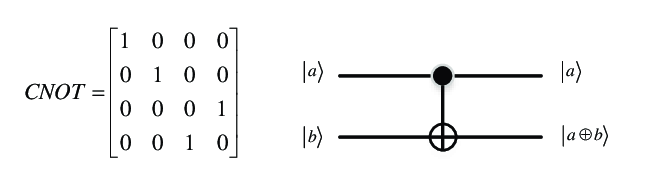
\includegraphics[width=\linewidth]{Matrix-representation-and-quantum-circuit-of-CNOT-gate.png}
	\caption{نمایش ماتریسی و نمایش گیت کوانتومی \lr{CNOT}}
	\label{CNOT}
\end{figure}


در شکل بالا گیت \lr{CNOT} در مدار کوانتومی به تصویر درآمده است. کیوبیت کنترل شده  حالت $\vert a \rangle$ و کیوبیت هدف حالت $\vert b \rangle$ می‌باشد.


با اعمال این عملگر به حالت $\vert 10\rangle$ داریم:
$$
\text{CNOT} \ket{10} = \begin{pmatrix}
	1 & 0 & 0 & 0 \\
	0 & 1 & 0 & 0 \\
	0 & 0 & 0 & 1 \\
	0 & 0 & 1 & 0
\end{pmatrix} \begin{pmatrix}
	0 \\
	0 \\
	1 \\
	0
\end{pmatrix} = \begin{pmatrix}
	0 \\
	0 \\
	0 \\
	1
\end{pmatrix} = \ket{11}
$$\\
این فرآیند به صورت معکوس نیز قابل رخ دادن است:\\

$$
\text{CNOT} \ket{11} = \begin{pmatrix}
	1 & 0 & 0 & 0 \\
	0 & 1 & 0 & 0 \\
	0 & 0 & 0 & 1 \\
	0 & 0 & 1 & 0
\end{pmatrix} \begin{pmatrix}
	1 \\
	1 \\
	0 \\
	0
\end{pmatrix} = \begin{pmatrix}
	0 \\
	1 \\
	0 \\
	0
\end{pmatrix} = \ket{10}
$$
از این گیت کوانتومی‌، برای بسیاری مدار‌ها و شبیه‌سازی‌های کوانتومی، از جمله تلپورت، درهمتنیدگی و ...،استفاده می‌شود.

\subsection*{گیت تغییر فاز}
گیت تغییر فاز که به آن گیت P یا گیت فاز نیز می گویند، یک کیوبیت است.
دروازه ای که فاز نسبی را بین دو بردار پایه جابجا می کند. به عنوان زیر تعریف شده است:
\begin{center}
	\begin{equation}
		\begin{aligned}
		& \boldsymbol{U}_{\boldsymbol{PS}, \boldsymbol{\phi}}|0\rangle=|0\rangle \\
		& \boldsymbol{U}_{\boldsymbol{PS},  \boldsymbol{\phi}}|1\rangle=e^{i \Phi}|1\rangle
	\end{aligned}
\end{equation}
\end{center}


که در آن $\Phi$ فاز و $e^{i\Phi}$ عامل فاز است. 
زمانی که گیت تغییر فاز بر حالت $\vert 0 \rangle$  اثرکند، هیچ تغییری حاصل نمی‌شود. اما با اعمال این گیت به بردار حالت $\vert 1 \rangle$، یک فاز اضافه به بردار افزوده خواهد شد. برای افزدون فاز اضافه  باید یک عامل نظیر  $e^{i\Phi}$ در بردارد حالت ضرب شود. برای درک بهتر مطلب باید به حالت ماتریسی این گیت رجوع کنیم.





\subsubsection{نمایش ماتریسی گیت تغییر فاز}

نمایش ماتریسی گیت تغییر فاز $\boldsymbol{U}_{\boldsymbol{P} \boldsymbol{S}, \boldsymbol{\Phi}}$ به صورت زیر است:

\begin{center}
	$$\boldsymbol{U}_{\boldsymbol{P} \boldsymbol{S}, \boldsymbol{\Phi}}=\left(\begin{array}{cc}
		1 & 0 \\
		0 & e^{i \Phi}
	\end{array}\right)$$
\end{center}
با استفاده از روابط بالا می‌توان  به راحتی اثبات کرد: 
\begin{center}
	$$U_{P S, \boldsymbol{\phi}}|1\rangle=\left(\begin{array}{cc}
		1 & 0 \\
		0 & e^{i \Phi}
	\end{array}\right)\left(\begin{array}{l}
		0 \\
		1
	\end{array}\right)=\left(\begin{array}{c}
		0 \\
		e^{i \Phi}
	\end{array}\right)=e^{i \Phi}\left(\begin{array}{l}
		0 \\
		1
	\end{array}\right)=e^{i \Phi}|1\rangle$$
\end{center}




\subsubsection{گیت تغییر فاز در مدار و خصوصیات آن}
درحالت کلی برای سیستم های تک کیوبیتی می‌توان نوشت:

\begin{center}
	$$\begin{aligned}
		\boldsymbol{U}_{\boldsymbol{P S}, \boldsymbol{\Phi}}|\Psi\rangle & =\left(\begin{array}{cc}
			1 & 0 \\
			0 & e^{i \Phi}
		\end{array}\right)\left(\begin{array}{l}
			\alpha \\
			\beta
		\end{array}\right)=\left(\begin{array}{c}
			\alpha \\
			e^{i \Phi} \beta
		\end{array}\right) \\
		& =\alpha|0\rangle+e^{i \Phi} \beta|1\rangle
	\end{aligned}$$
\end{center}
در بردار اصلی، $\alpha$ و $\beta$ اعداد مختلط می‌باشند؛ به همین دلیل این اعداد را می‌توان به به عنوان یک ضریب فاز معرفی کرد:

\begin{center}
\begin{equation}
\alpha = e^{i\theta_{1} \vert\alpha\vert }, \beta = e^{i\theta_{2} \vert\beta\vert}
\end{equation}
\end{center}
که در آن $\theta1$ و $\theta2$ به ترتیب فازهای $\alpha$ و $\beta$ هستند.

\textbf{اشکال}
بنابراین، اختلاف فاز آنها θ1 - θ2 است. با توجه به رفتارگیت تغییر فاز، تغییر فاز $\alpha$ صفر می‌باشد؛‌اما فاز β به Φ + θ2 تغییر می کند. بنابراین، خویشاوندان آنها فاز با Φ تغییر می کند. 

\begin{latin}
	\begin{center}
		This also explains why the phase shift is only applied to the
		second basis state to be meaningful. If it is applied to both, there will be no change
		in the phase difference.
	\end{center}
\end{latin}


 (1 0
0 e iπ
)
=
(1 0
0-1
)
زیرا e iπ = cos π + i sin π = -1.



 این ماتریس پائولی $ \sigma_{z}$ می‌باشد؛ که به آن Z-gate نیز می گویند. گیت تغییر فاز، فاز نسبی $vert 0 \rangle$و |1〉 را با Φ تغییر می دهد. و به این ترتیب گیت $Z$ فاز نسبی را با $\pi$ تغییر می دهد. 
 
 
 
\subsection{گیت مبادله}
یک گیت مبادله\footnote{\lr{Swap gate}} اعداد را در حالت های پایه یک رجیستر 2 کیوبیتی جابجا می کند. اگر فقط حالت های پایه را در نظر بگیریم، معادل مبادله حالات دو الکترون است. این گیت به صورت  زیر تعریف می‌شود:
\begin{center}
\begin{equation}
	U_{SWAP}   \vert ab\rangle = \vert ba \rangle
\end{equation}
\end{center}
که در آن a و b فقط اعداد کیوبیت اول و دوم در پایه هستند. a و b می‌توانند مقادیر 0 و 1 را اتخاذ کنند. بنابرین می‌توان نوشت:
\begin{center}
	$$\begin{aligned}
		& U_{S W A P}|00\rangle=|00\rangle \\
		& U_{S W A P}|01\rangle=|10\rangle \\
		& U_{S W A P}|10\rangle=|01\rangle \\
		& U_{S W A P}|11\rangle=|11\rangle
	\end{aligned}$$
\end{center}




بنابراین، تنها $\vert 01 \rangle$ و $\vert 10 \rangle$ تحت مبادله (به یکدیگر) تغییر می کنند.
اعمال این گیت برای حالات $\vert 00 \rangle$ و $\vert 11 \rangle$، بدون اثر است؛ زیرا "0" و "0" یا "1" و "1" تعویض می‌شوند؛ که پیامد خاصی در پی ندارد.


\subsubsection{نمایش ماتریسی گیت مبادله}
نمایش ماتریسی $U_{S W A P}$ به شکل زیر است:
\begin{center}
	$$U_{S W A P}=\left(\begin{array}{llll}
		1 & 0 & 0 & 0 \\
		0 & 0 & 1 & 0 \\
		0 & 1 & 0 & 0 \\
		0 & 0 & 0 & 1
	\end{array}\right)$$
\end{center}
\
 از آنجایی که این یک گیت 2 کیوبیتی برای عملیات است یک بردار در فضای چهار بعدی $\mathbb{c}^4$، ماتریس (یا عملگر) باید 4 × 4 باشد. علاوه بر این، فقط حالت پایه دوم و سوم را جابجا می کند. بنابراین، تنها ردیف دوم و سوم با ماتریس یکه متفاوت هستند. به طور مثال:
\begin{center}
	$$U_{S W A P}|10\rangle=\left(\begin{array}{llll}
		1 & 0 & 0 & 0 \\
		0 & 0 & 1 & 0 \\
		0 & 1 & 0 & 0 \\
		0 & 0 & 0 & 1
	\end{array}\right)\left(\begin{array}{l}
		0 \\
		0 \\
		1 \\
		0
	\end{array}\right)=\left(\begin{array}{l}
		0 \\
		1 \\
		0 \\
		0
	\end{array}\right)=|01\rangle$$
\end{center}
این رابطه‌ بصورت معکوس نیز برقرارست.

\subsubsection{گیت مبادله در مدار و خصوصیات آن}
به طور کلی، برای یک بردار 2 کیوبیتی، نظیر $\vert \Psi \rangle=\alpha|00\rangle+\gamma|01\rangle+\beta|10\rangle+\delta|11\rangle$ داریم:

\begin{center}
	$$\begin{aligned}
		\boldsymbol{U}_{\boldsymbol{SWAP}}|\Psi\rangle & =\left(\begin{array}{llll}
			1 & 0 & 0 & 0 \\
			0 & 0 & 1 & 0 \\
			0 & 1 & 0 & 0 \\
			0 & 0 & 0 & 1
		\end{array}\right)\left(\begin{array}{l}
			\alpha \\
			\beta \\
			\gamma \\
			\delta
		\end{array}\right)=\left(\begin{array}{l}
			\alpha \\
			\gamma \\
			\beta \\
			\delta
		\end{array}\right) \\
		\vspace{2cm}
		& =\alpha|00\rangle+\gamma|01\rangle+\beta|10\rangle+\delta|11\rangle
	\end{aligned}$$
\end{center}





\begin{figure}[ht]
	\centering
	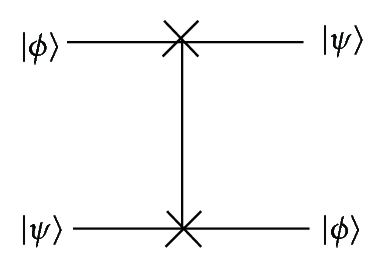
\includegraphics[width=50mm,scale=0.5]{swap.png}
	\caption{نمایش گیت کوانتومی مبادله در مدار کوانتومی}
	\label{SWAP}
\end{figure}



همانطور که انتظار می رود، ضرایب حالت های پایه دوم و سوم با هم مبادله می شوند.
\section{مدار‌های کوانتومی}
مدار‌های ‌کوانتومی\footnote{quantum circuit}، یک دسته از گیت ها‌ی کوانتومی،که با یک توالی بخصوص قرار گرفته اند، ‌می‌باشند. این کیوبیت ها، با توالی یاد شده، روی یک یا چند دسته کیوبیت، اثر داده ‌می‌شوند. 

مدار‌های کوانتومی، یکی از اولین مفهوم‌های بکار‌رفته برای تعریف کامپیوتر‌های کوانتومی‌ می‌باشند. برای تعریف و شبیه‌سازی هریک از پدیده‌ها و الگوریتم‌های کوانتومی، نیاز به پیاده‌سازی یک مدار به‌خصوص داریم.


مدارهای کوانتومی یک ابزار قدرتمند برای محاسبات کوانتومی هستند. آنها می توانند برای پیاده سازی طیف گسترده ای از الگوریتم های کوانتومی، از جمله الگوریتم شاور برای رمزگشایی اعداد صحیح و الگوریتم گروور برای جستجوی پایگاه داده های بدون ترتیب استفاده شوند.


\begin{figure}[htbp]
	\centering
	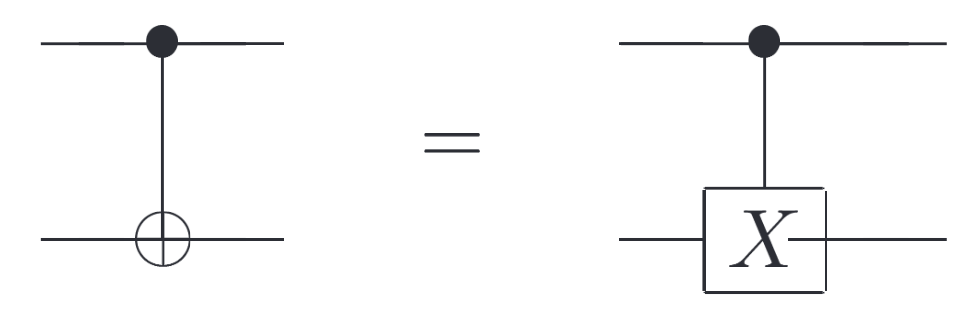
\includegraphics[width=\linewidth]{cnot in circuit.png}
	\caption{نمایش‌های مختلف گیت CNOT در مدار کوانتومی}
	\label{fig:my_image}
\end{figure}

یکی دیگر از عملگر‌های مهم در مدار کوانتومی، عملگر اندازه‌گیری است. که در شکل زیر نشان داده شده است. همانطور که پیش از این بیان شد؛ در بردار حالت $\vert \Psi \rangle = \alpha \vert 0 \rangle + \beta \vert 1 \rangle$ هنگام مشاهده به یک حالت کلاسیکی رمبش می‌کند؛‌احتمال اینکه به حالت $\vert 0 \rangle$رمبش کند، $\vert \alpha \vert ^2$, و احتمال اینکه به حالت $\vert 1 \rangle$ رمبش کند، $\vert \beta \vert ^2$، می‌باشد.

 
\begin{figure}[ht]
	\centering
	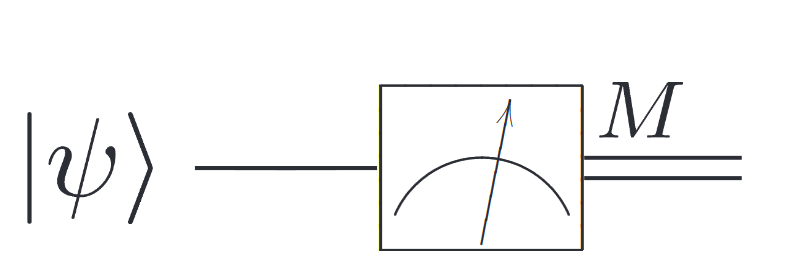
\includegraphics[width=\linewidth, scale=0.5]{measurment.png}
	\caption{نمایش‌های مختلف گیت CNOT در مدار کوانتومی}
	\label{fig:my_image}
\end{figure}


مدار‌های کوانتومی مدلی بسیار سودمند برای شبیه‌سازی‌ فرآیندهای کوانتومی‌ است. این فرآیندها محدود به عملیات‌های محاسباتی نخواهد شد؛ بلکه در اغلب حوزه‌‌ها اعم از ارتباطات، اختلالات کوانتومی\footnote{quantum noise} و ... بکار‌خواهدرفت.
\subsubsection{شباهت ها و تفاوت های مدارهای کلاسیک و کوانتومی}
مدارهای کوانتومی مشابه مدارهای کلاسیک هستند، اما از دروازه های کوانتومی به جای دروازه های منطقی کلاسیک استفاده می کنند. دروازه های کوانتومی عملیات قابل برگشت هستند که می توانند برای دستکاری حالت کوانتومی یک کیوبیت استفاده شوند.

\textbf{شباهت ها}

\begin{itemize}
	\item هر دو مدار کوانتومی و کلاسیک از یک دنباله عملیاتی تشکیل شده اند که به یک مجموعه داده اعمال می شوند.
	\item هر دو مدار را می توان به صورت گرافیکی با نماد مشابهی نشان داد.
	\item هر دو مدار می توانند برای پیاده سازی الگوریتم ها استفاده شوند.
\end{itemize}

\textbf{تفاوت ها}

\begin{itemize}
	\item مدارهای کوانتومی از کیوبیت ها، که معادل کوانتومی مفهوم بیت هستند، به عنوان واحد پایه داده خود استفاده می کنند. 
	\item مدارهای کلاسیک از بیت ها ، که بیت های کلاسیک هستند ، به عنوان واحد پایه داده خود استفاده می کنند.
	\item مدارهای کوانتومی از دروازه های کوانتومی ، که عملیات قابل برگشت هستند ، به عنوان عملیات پایه خود استفاده می کنند.
	\item  مدارهای کلاسیک از دروازه های منطقی ، که عملیات برگشت ناپذیر هستند ، به عنوان عملیات پایه خود استفاده می کنند.
	\item مدارهای کوانتومی می توانند خواص مکانیک کوانتوم را ، مانند برهمنهی و درهمتنیدگی ، برای انجام کارهایی که برای رایانه های کلاسیک غیرممکن است ، بهره مند شوند.
\end{itemize}


\renewcommand{\arraystretch}{1.5}
\begin{table}[ht]
	\centering
	\begin{tabular}[5pt]{|p{100pt}|p{100pt}|p{100pt}|}
		\hline
		\textbf{ویژگی} & \textbf{مدار کوانتومی} &\textbf{مدار کلاسیک} \\
		\hline
		واحد پایه داده & کیوبیت & بیت \\
		\hline
	      عملیات پایه & دروازه های کوانتومی & دروازه های منطقی \\
		\hline
		برگشت پذیری & قابل برگشت & برگشت ناپذیر \\
		\hline
	\end{tabular}
	\caption{شباهت‌ها و تفاوت های مدارهای کلاسیک و کوانتومی}
\end{table}



\subsubsection{اجزای مدار‌های کوانتومی و سایز آن }
\paragraph{اندازه مدار کوانتومی}

اندازه یک مدار کوانتومی تعداد دروازه های موجود در مدار است. پیچیدگی یک الگوریتم کوانتومی اغلب با اندازه مدار کوانتومی مورد نیاز برای پیاده سازی آن اندازه گیری می شود.


\paragraph{کیوبیت}

کیوبیت ها واحد پایه اطلاعات در محاسبات کوانتومی هستند. آنها می توانند در یک برهنهی کوانتومی از دو حالت ، 0 و 1 باشند. این بدان معنی است که یک کیوبیت می تواند هم 0 و هم 1 باشد ، که یک ویژگی به نام برهمنی کوانتومی است. کیوبیت ها همچنین می توانند به هم متصل شوند ، که به این معنی است که حالت یک کیوبیت به حالت کیوبیت دیگر وابسته است.
\paragraph{دروازه}
دروازه ها عملیاتی هستند که روی کیوبیت ها اعمال می شوند. آنها می توانند برای ایجاد برهمنهی ، انجام چرخش ها و درهم تنیدگی کیوبیت ها استفاده شوند. انواع مختلفی از دروازه ها وجود دارد ، اما برخی از رایج ترین آنها شامل گیت هادامارد ، گیت CNOT و گیت توفولی است.

\paragraph{عملیات}

عملیات اقداماتی هستند که روی کیوبیت ها انجام می شوند. آنها می توانند اندازه گیری ها یا سایر اقدامات باشند. اندازه گیری ها برای رمبش حالت کوانتومی یک کیوبیت به یک مقدار قطعی ، 0 یا 1 استفاده می شود.



اجزای اساسی یک مدار کوانتومی کیوبیت ها ، دروازه ها و عملیات هستند. این اجزا برای ایجاد الگوریتم های کوانتومی استفاده می شوند که الگوریتم هایی هستند که فقط می توانند روی یک رایانه کوانتومی اجرا شوند. مدارهای کوانتومی یک ابزار قدرتمند برای محاسبات کوانتومی هستند و پتانسیل انقلابی در بسیاری از زمینه های مختلف ، از جمله رمزنگاری ، شیمی و یادگیری ماشین را دارند.

\subsection{نحوه‌ی نمایش مدار‌های کوانتومی}


مدارهای کوانتومی با استفاده از نماد گرافیکی مشابه نمودارهای مدار استفاده شده در محاسبات کلاسیک نوشته می شوند. محور افقی یک مدار کوانتومی زمان را نشان می دهد و محور عمودی کیوبیت ها را نشان می دهد. دروازه ها توسط جعبه ها نشان داده می شوند و خطوط بین جعبه ها نشان دهنده ارتباطات بین کیوبیت ها است.

\begin{figure}[ht]
	\centering
	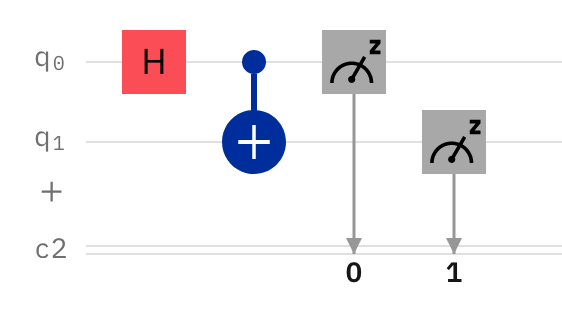
\includegraphics[]{meas-firstcirc.png}
	\caption{مدارکوانتومی شبیه‌سازی شده برای آزمایش درهمتنیدگی}
\end{figure}

\chapter{برنامه‌نویسی کوانتومی}
برنامه نویسی کوانتومی فرآیند طراحی و پیاده‌سازی دنباله هایی از دستورالعمل هایی موسوم مدارهای کوانتومی می‌باشد، با استفاده از گیت ها، سوئیچ ها و عملگرها برای دستکاری وضعیت کوانتومی یک کیوبیت به پردازش مسائل می‌پردازیم.

مدارهای کوانتومی یک نمایش گرافیکی از الگوریتم های کوانتومی هستند، این الگوریتم هایی فقط روی یک کامپیوتر کوانتومی قابل اجرا هستند.

برنامه نویسی کوانتومی یک زمینه نسبتاً جدید است و تعدادی زبان برنامه نویسی کوانتومی مختلف در دسترس است. برخی از محبوب ترین زبان های برنامه نویسی کوانتومی عبارتند از \lr{Qiskit}، \lr{Cirq} و \lr{Quil}.

برنامه نویسی کوانتومی یک زمینه پیچیده و چالش برانگیز است، اما این پتانسیل را دارد که در بسیاری از زمینه های مختلف از جمله رمزنگاری، شیمی و یادگیری ماشین انقلابی ایجاد کند. با قدرتمندتر شدن کامپیوترهای کوانتومی، برنامه نویسی کوانتومی اهمیت فزاینده ای پیدا خواهد کرد.
\section{کامپیوترهای کوانتومی در مقابل کامپیوترهای کلاسیک}



کامپیوترهای کوانتومی و کامپیوترهای کلاسیک دو نوع بسیار متفاوت از رایانه هستند. کامپیوترهای کوانتومی از بیت‌های کوانتومی (کیوبیت‌ها) برای ذخیره اطلاعات استفاده می‌کنند، در حالی که کامپیوترهای کلاسیک از بیت‌ها استفاده می‌کنند. کیوبیت‌ها می‌توانند در حالت برهم‌نهی دو حالت، 0 و 1، به‌طور همزمان باشند، در حالی که بیت‌ها فقط می‌توانند در یک حالت به‌طور همزمان باشند. این تفاوت در نحوه ذخیره اطلاعات امکان محاسباتی را برای کامپیوترهای کوانتومی فراهم می‌کند که برای کامپیوترهای کلاسیک غیرممکن است.

علاوه بر تفاوت در نحوه ذخیره اطلاعات، کامپیوترهای کوانتومی و کلاسیک در نحوه انجام محاسبات نیز متفاوت هستند. کامپیوترهای کوانتومی از مکانیک کوانتوم برای انجام محاسبات استفاده می‌کنند، در حالی که کامپیوترهای کلاسیک از منطق بولی استفاده می‌کنند. این تفاوت در نحوه انجام محاسبات نیز به کامپیوترهای کوانتومی امکان می‌دهد تا برای برخی از وظایف، محاسباتی را بسیار سریع‌تر از کامپیوترهای کلاسیک انجام دهند.

کاربردهای بالقوه کامپیوترهای کوانتومی بسیار گسترده است. آنها می‌توانند برای رمزگشایی روش‌های رمزنگاری فعلی، شبیه‌سازی مولکول‌ها و آموزش مدل‌های یادگیری ماشینی که بسیار دقیق‌تر از مدل‌های فعلی هستند، استفاده شوند. کامپیوترهای کوانتومی هنوز در مراحل اولیه توسعه هستند، اما پتانسیل تغییر جهان را دارند. هنگامی که کامپیوترهای کوانتومی قدرتمندتر شوند، قادر به حل مشکلاتی خواهند بود که برای کامپیوترهای کلاسیک در حال حاضر غیرممکن است.

 برخی از مثال‌های خاص از نحوه استفاده از کامپیوترهای کوانتومی:

\paragraph{رمزنگاری}: کامپیوترهای کوانتومی می‌توانند برای رمزگشایی روش‌های رمزنگاری فعلی استفاده شوند، که تأثیر عمده‌ای بر امنیت آنلاین خواهد داشت.
\paragraph{شبیه‌سازی مواد در علم شیمی}:کامپیوترهای کوانتومی می‌توانند برای شبیه‌سازی مولکول‌ها استفاده شوند، که می‌تواند به دانشمندان در توسعه داروها و مواد جدید کمک کند.
\paragraph{یادگیری ماشینی}: کامپیوترهای کوانتومی می‌توانند برای آموزش مدل‌های یادگیری ماشینی که بسیار دقیق‌تر از مدل‌های فعلی هستند، استفاده شوند.

آینده محاسبات کوانتومی بسیار روشن است. هنگامی که کامپیوترهای کوانتومی قدرتمندتر شوند، قادر به حل مشکلاتی خواهند بود که برای کامپیوترهای کلاسیک در حال حاضر غیرممکن است. این می‌تواند منجر به پیشرفت‌های عمده در بسیاری از زمینه‌های مختلف شود.
\section{شبیه‌سازی کلاسیک در مقابل کامپیوتر کوانتومی}
% computer vs simulator https://www.youtube.com/watch?v=2qcvgXaDdfU
% https://www.youtube.com/watch?v=0RPFWZj7Jm0	

بسیاری از مسائل کوانتومی و بسیاری از الگوریتم‌های کوانتومی قابل شبیه‌سازی روی کامپیوتر‌های کوانتومی می‌باشند. بنابرین یک سوال به‌واقع مهم مطرح می‌شود: \textbf{چرا به یک کامپیوتر کوانتومی نیاز داریم؟}

در هنگام محاسبات کوانتومی،‌ کامپیوتر‌های کلاسیک دارای محدودیت‌هایی هستند. به طور مشابه کامپیوتر‌های کوانتومی نیز دارای معایبی هستند؛ که قابل بحث و بررسی هستند. دراین بخش به این مزایا و معایب هرکدام از کامپیوترها می‌پردازیم و در ادامه به اهداف تعریف شده برای کامپیوترهای کوانتومی می‌پردازیم.


\subsection{تفاوت کامپیوترهای کوانتومی و شبیه‌سازهای کلاسیک}
همانطور که در بخش‌های قبلی گفته شد؛ کامپیوترهای کوانتومی با استفاده از کیوبیت‌ها تعریف می‌شوند. یک کیوبیت به صورت یک ترکیب خطی از حالت $\vert0\rangle$ و $\vert1\rangle$ تعریف می‌شود:

\begin{center}
\begin{equation}
\vert\psi\rangle = \alpha\vert0\rangle + \beta\vert1\rangle
\end{equation}
\end{center}

هریک از حالات داخل رابطه‌ی بالا به صورت یک ماتریس قابل تعریف هستند. به طور مشابه هریک از عملگر های کوانتومی را می‌توان به صورت یک ماتریس تعریف کرد. ماتریس‌هایی مشابه ماتریس پائولی یا در مقیاس‌های بالاتر ماتریس فردکین که برای سه کیوبیت تعریف می‌شود؛ و محاسبات را سریع می‌سازد.



از طرفی دیگر تعداد محاسبات در مدار‌های کلاسیک به تعداد حالات مسأله بستگی دارد. در محاسبات کلاسیک هرچه تعداد حالات بالاتر برود؛ پیچیدگی محاسبات بالاتر‌می‌رود و حتی اغلب با حالت نمایی رشد می‌کنند. این درحالیست که در محاسبات کوانتومی هر یک حالات مختلف مسأله به یک دنیای موازی کوانتومی شیفت داده می‌شود و از این طریق محاسبات به زمان و منابع کمتری نیاز دارد.


مهم‌ترین عامل در سطح پیچیدگی محاسبات کوانتومی همدوسی می‌باشد. 
همدوسی در محاسبات کوانتومی اصلی ترین منبع خطا در این سیستم ها است. کیوبیت ها بسیار به محیط خود هستند و می توانند به راحتی توسط  تعامل با فوتون ها، الکترون ها و سایر ذرات با آن‌ها دچار ناهمدوسی شوند. این می تواند باعث شود که کیوبیت ها خواص کوانتومی خود را مانند برهمنهی کوانتومی و درهمتنیدگی که برای انجام محاسبات کوانتومی ضروری هستند، از دست بدهند.

ناهمدوسی می‌تواند به دلایل مختلفی ایجاد شود:

\paragraph{دما}کیوبیت ها در دماهای بالاتر مستعد دکوراسیون هستند. این به این دلیل است که هرچه دما بالاتر باشد، کیوبیت ها انرژی بیشتری دارند و بیشتر احتمال دارد با محیط خود تعامل داشته باشند.

\paragraph{برخورد}کیوبیت ها همچنین می توانند توسط ارتعاشات دکور شوند. این به این دلیل است که ارتعاشات می توانند باعث حرکت کیوبیت ها شوند، که می تواند حالت های کوانتومی آنها را مختل کند.

\paragraph{تابش الکترومغناطیسی}کیوبیت ها می توانند توسط تابش الکترومغناطیسی، مانند نور و امواج رادیویی، دکور شوند. این به این دلیل است که تابش الکترومغناطیسی می تواند با الکترون های کیوبیت ها تعامل داشته باشد و باعث از دست رفتن خواص کوانتومی آنها شود.

ناهمدوسی یک مانع بزرگ برای توسعه ابررایانه های کوانتومی است. برای ساخت یک رایانه کوانتومی عملی، باید راه هایی برای کاهش ناهمدوسی پیدا کرد. این یک مشکل بزرگ ولی قابل حل است؛ اما تعدادی از مسیرهای تحقیقاتی امیدوار کننده وجود دارد، مانند:

\paragraph{سردسازی کیوبیت‌ها} این می تواند انرژی کیوبیت ها را کاهش دهد و آنها را کمتر مستعد تعامل با محیط خود کند.

\paragraph{استفاده از مواد با همدوسی بالا}برخی از مواد، مانند ابررساناها، زمان های همدوسی بسیار طولانی دارند که آنها را برای استفاده در رایانه های کوانتومی بسیار مناسب می کند.

\paragraph{توسعه‌ی الگوریتم‌های جایگزین برای تصحیح خطای‌‌کوانتومی}
الگوریتم های تصحیح خطا کوانتومی می توانند برای تشخیص و تصحیح خطاهایی که توسط ناهمدوسی ایجاد می شوند استفاده شوند.

\section{کامپیوترکوانتومی IBM و زبان برنامه‌نویسی QisKit}\label{sec:Qiskit}

\subsection{معرفی QisKit}
یک زبان برنامه‌نویسی کوانتومی است. این زبان دارای مشابهت‌های زیادی با زبان پایتون می‌باشد. دو دلیل عمده برای این شباهت وجود دارد:\\
 1. این زبان براساس زبان پایتون و برخی کتابخانه‌های آن ساخته شده است. \\
 2. جامعه دانشمندان کوانتوم و به‌طور کلی فیزیکدانان از سابق برای انجام شبیه‌سازی‌های خود از زبان پایتون استفاده می‌کنند و پایتون نیز کتابخانه‌هاي بسیار کارآمدی - نظیر نامپای\footnote{Numpy} ، پانداس\footnote{Pandas} ، سایپای\footnote{Scipy} و .. - ارائه کرده است.

\subsection{کدنویسی به زبان QisKit}
برای کدنویسی به زبان \lr{QisKit} می‌توان از محیط \lr{Jupyter notebook} استفاده کرد. پس از نصب \lr{Qiskit} برای فرخواندن این کتابخانه به راحتی می‌توان نوشت:

\begin{latin}
	\begin{verbatim}
		import qiskit
	\end{verbatim}
\end{latin}

هدف از برنامه نویسی کوانتومی پیاده‌سازی مسائل کوانتومی روی کامپیوتر‌کوانتومی‌ واقعی است. بدین منظور ابتدا یک شبیه سازی روی سیستم خود انجام داده و سپس کد خود را به کامپیوتر‌کوانتومی \lr{IBM} ارسال می‌کنیم.بدین منظور می‌بایست یک حساب کاربری در سایت مرتبط به کامپیوتر کوانتومی \lr{IBM} ایجاد کنیم.


\subsection{قواعد نوشتاری و ساختار داده}
هرزبان برنامه نویسی دارای ساختار داده و دستورات نگارشی مخصوص به‌خود است؛ \lr{QisKit} نیز از این قاعده مستثنی نیست. بدین دلیل در ادامه به اختصار به معرفی برخی دستورات این زبان می‌پردازیم. باید خاطر نشان کرد که این متن براساس \lr{QisKit} نسخه‌ی  0.44.0 نوشته‌ شده‌است.

هدف نهایی این برنامه‌ها، پیاده‌سازی یک مدار کوانتومی‌ منتسب به یک مسئله‌ی خاص است. پس نیاز به تعریف و ایجاد کیوبیت داریم. برای تعریف کیوبیت از راه زیر استفاده می‌کنیم:

\begin{latin}
	\begin{verbatim}
		quantum_register = QuantumRegister(n)
	\end{verbatim}
\end{latin}
که در آن n تعداد کیوبیت‌های داخل کوانتوم رجیستر مدنظر برنامه نویس است.


\begin{latin}
	\begin{verbatim}
		classic_register = ClassicalRegister(n)
	\end{verbatim}
\end{latin}
که در آن n تعداد بیت‌های داخل رجیستر کلاسیک مدنظر برنامه نویس است.


درنهایت ‌می‌توان با قرار دادن این دو رجیستر‌ایجاد شده،‌ در یک مدار، یک مدار کوانتومی ایجاد کنیم:


\begin{latin}
	\begin{verbatim}
		circuit = QuantumCircuit(quantum_register, classic_register)
	\end{verbatim}
\end{latin}


پس از ایجاد مدار می‌توان عملگر‌های مدنظر خود نظیر هادامارد و \lr{CNOT} و ... را روی بخش‌های مختلف مدار اثر داد.
از طرفی می‌توان مدار ایجاد شده را به صورت یک تصویر به کاربر نشان داد.


\subsection{پیاده‌سازی گیت‌های کوانتومی}
برای اعمال یک گیت کوانتومی روی اجزای یک مدار کوانتومی،‌ابتدا باید نام مدار کوانتومی را نوشت؛ سپس نام گیت کوانتومی را نوشت؛ سپس نام کیوبیت یا بیت مدنظر را نوشت: 

\begin{latin}
	\begin{verbatim}
		circuit.gate_sing_inQisKit(Qubit_name, Bit_name)
	\end{verbatim}
\end{latin}


در کد بالا به جای \lr{gate\_sing\_inQisKit()} نام هر گیت کوانتومی مدنظر برنامه‌نویس می‌تواند باشد.

\pagebreak
\subsection{تصویر سازی}

برای تصویر کردن وضعیت مدار کوانتومی می‌بایست از راه زیر استفاده کرد:

\begin{latin}
\begin{verbatim}
# to run commands and show diagram in a easier way.
%matplotlib inline 

# draw circuit
circuit.draw()

# we can change look of diagram.
circuit.draw(output = "mpl")  # output = "mpl" is defining type of circuit output

\end{verbatim}
\end{latin}

درنهایت خروجی مشابه خروجی های زیر را می‌توان از این زبان برنامه نویسی دریافت کرد:

\begin{center}
\begin{figure}[h]
\centering
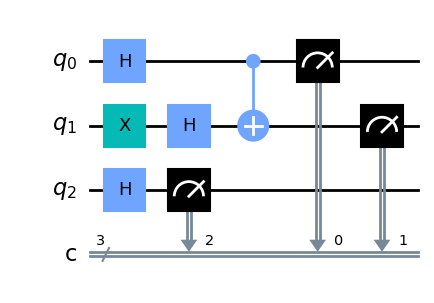
\includegraphics[]{tutorials_circuits_advanced_03_advanced_circuit_visualization_7_0.png}
\caption{نمونه‌ای از خروجی کیس‌کیت}
\end{figure}
\end{center}
\let\cleardoublepage\clearpage
\chapter{الگوریتم‌های‌کوانتومی‌}


چه گونه‌ای از مسائل محاسباتی قابل اجرا با مدارهای کوانتومی می‌باشند؟ 
تفاوت و برتری مدار‌های کوانتومی نسبت به مدار‌های کلاسیک چیست؟
آیا می‌توان یک حوزه‌ی خاص را تعیین کرد؛ به گونه‌ای که عملکرد کامپیوترهای‌‌کوانتومی نسبت به کامپیوتر‌های کلاسیک مزیت داشته باشند؟

در این بخش می‌خواهیم به طور خلاصه این سوالات را پاسخ دهیم و توضیح دهیم چگونه می‌توان از کامپیوتر‌های کوانتومی به شکلی سودمند استفاده کنیم.

\section{موازی سازی کوانتومی}

موازی‌سازی کوانتومی\footnote{Quantum parallelism}، پایه‌واساس بسیاری از الگوریتم‌های کوانتومی است. با گذار یک حالت کوانتومی به حالت برهمنهی کوانتومی، درحین محاسبات کوانتومی یک تابع نظیر \lr{f(x)}، می‌تواند مقادیر مختلف \lr{x} را به طور همزمان بررسی کند. این درحالیست که در محاسبات کلاسیک به دلیل ماهیت بیت‌های اطلاعات، تابع \lr{f(x)} فقط می‌تواند یکی از مقادیر مجاز برای \lr{x} را بررسی کند.


فرض کنید تابع f ،یک تابع تک-کیوبیت، به صورت زیر تعریف شده است:\\
\begin{center}
\begin{equation}
f (x) : \{0, 1\} \rightarrow \{0, 1\}
\end{equation}
\end{center}

روش مناسب برای محاسبه این تابع در یک کامپیوتر کوانتومی، با در نظر گرفتن دو کیوبیت که در حالت $\vert x, y\rangle$شروع می شود. با یک توالی مناسب از گیت های منطقی می توان این حالت را به $\vert f(x) \oplus x, y\rangle$ تبدیل کرد که در آن $\oplus$ بیانگر جمع مدوله با پایه‌2 می‌باشد.

\footnote{Modulo 2 is a mathematical operation that returns the remainder of a division by 2. For example, 5 mod 2 is 1, because 5 divided by 2 has a quotient of 2 and a remainder of 1.
	
	The symbol "⊕" is often used to indicate addition modulo 2. So, the expression "5 ⊕ 3" would be evaluated as follows:
	
	5 ⊕ 3 = (5 + 3) mod 2 = 8 mod 2 = 0
	This is because 8 divided by 2 has a quotient of 4 and a remainder of 0.
	
	Modulo 2 is a useful operation in many different areas of mathematics, including cryptography, computer science, and number theory. It is also used in everyday life, for example, when checking whether a number is even or odd.
	
	Here are some other examples of modulo 2:
	
	1 mod 2 = 1
	2 mod 2 = 0
	3 mod 2 = 1
	4 mod 2 = 0
	5 mod 2 = 1}

هریک از دسته‌های کیوبیت، \textbf{رجیستر کوانتومی} نامیده‌می‌شوند. اولین رجیستر، «رجیستر داده» و دومین رجیستر «رجیستر هدف» نامیده می‌شود.\\
ازین پس در این بخش به عامل گذار $\vert x, y \rangle \rightarrow \vert x, y \oplus f(x) \rangle$، عنوان «تابع \lr{$U_{f}$}» را اطلاق خواهیم کرد. لازم به ذکرست که این تبدیل، یک تبدیل یکه به شمار می‌آید.\footnote{اثبات این مطلب از حوصله‌ی بحث خارج است.}


اگر \lr{y = 0} آنگاه مقدار دومین کیوبیت بعد از اعمال تابع \lr{$U_{f}$} برابر با مقدار \lr{f(x)} خواهد بود.

 \begin{center}
 	 \begin{figure}[ht]
 		\centering
 		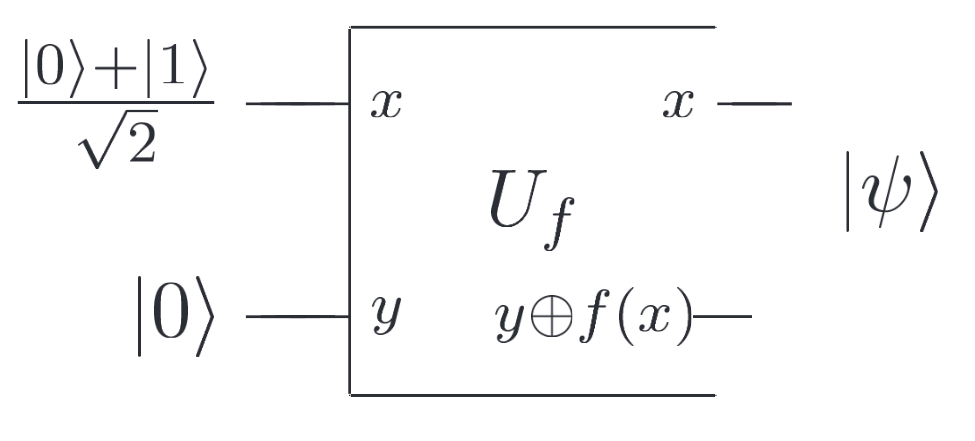
\includegraphics[width=0.8\textwidth]{Uforacle.png}
 		\caption{مدار کوانتومی برای ارزیابی $f (0)$ و $f (1)$ به طور همزمان. Uf مدار کوانتومی است که ورودی هایی مانند $\vert x, y\rangle$ را به $\vert x, y \rangle \rightarrow \vert x, y \oplus f(x) \rangle$، تصویر می‌کند.}
 	\end{figure}
 \end{center}

در شکل بالا مقادیر ورودی داده شده به تابع \lr{$U_{f}$} در پایه‌های محاسباتی قرار ندارند. رجیستر داده در حالت برهمنهی  قرار دارد. این حالت برهمنهی را می‌توان با اعمال گیت هادامارد بر حالت کوانتومی $\vert 0 \rangle$ ایجاد کرد. پس از ایجاد این حالت، تابع \lr{$U_{f}$} را به حالت جدید اعمال می‌کنیم:
\begin{center}
\begin{equation}\label{key}
\frac{\vert 0,f(0) \rangle +\vert 1,f(1) \rangle }{\sqrt{2}}
\end{equation}
\end{center}

این یک حالت استثنایی است! جملات مختلف کسر بالا حاوی اطلاعاتی در مورد$ f (0)$ و$f (1)$ می‌باشند؛ به‌نحوی که انگار $f (x)$ را برای دو مقدار $x$ به طور همزمان ارزیابی کرده ایم، این ویژگی به "موازی  سازی کوانتومی" موسوم می‌باشد. بر خلاف موازی سازی کلاسیک، که در آن هر یک مدارهای متعددی دارند ساخته شده برای محاسبه $f (x)$ به طور همزمان اجرا می شوند، در اینجا برای ارزیابی تابع برای چندین مقدار $x$ به طور همزمان، یک مدار $f (x)$ (با قابلیت برهمنهی کوانتومی)استفاده می شود.

این فرآیند را می توان به راحتی  با استفاده از یک عمل کلی به نام تبدیل هادامارد، به توابعی با تعداد بیت دلخواه تعمیم داد. این عمل فقط تعداد $n$ گیت هادامارد است که به طور موازی روی $n $کیوبیت عمل می کنند.

برای مثال در شکل زیر؛ دو کیوبیت در حالت $\vert 0 \rangle$ آماده شده‌‌اند. پس از اعمال گیت‌های هادامارد بر روی این رجیستر به خروجی زیر خواهیم رسید: 

\begin{center}
\begin{equation}
\Biggl( \frac{\vert 0 \rangle + \vert 1 \rangle}{\sqrt{2}}\Biggl)\Biggl( \frac{\vert 0 \rangle + \vert 1 \rangle}{\sqrt{2}}\Biggl) = \frac{\textbar00\rangle + \textbar01\rangle + \textbar10\rangle + \textbar11\rangle}{\sqrt{2}}\
\end{equation}
\end{center}

از نماد $\operatorname{H} \otimes 2$ به عنوان نشانه‌ی عملکرد موازی دو گیت هادامارد استفاده می‌کنیم؛از علامت $\otimes$ به عنوان تانسور یاد می‌کنیم. به طور کلی نتایج اعمال موازی گیت هادامارد روی \lr{n} کیوبیت روی حالت کوانتومی برابرست با:

\begin{center}
\begin{equation}
\frac{1}{\sqrt{2}} \sum_{x} \vert x \rangle
\end{equation}
\end{center}


در اینجا، $\sum$ نشان دهنده جمع بر روی همه مقادیر ممکن \lr{x} است، و ما$\operatorname{H} \otimes n$  را برای نشان دادن این عمل می نویسیم.
اعمال تبدیل هادامارد روی یک بهمنهی کوانتومی برابر از همه حالت های محاسباتی تولید می کند؛ و با استفاده از فقط $n$ گیت، یک برهمنهی از $2n$ حالت تولید می کند.
\begin{center}
	\begin{figure}[ht]
		\centering
		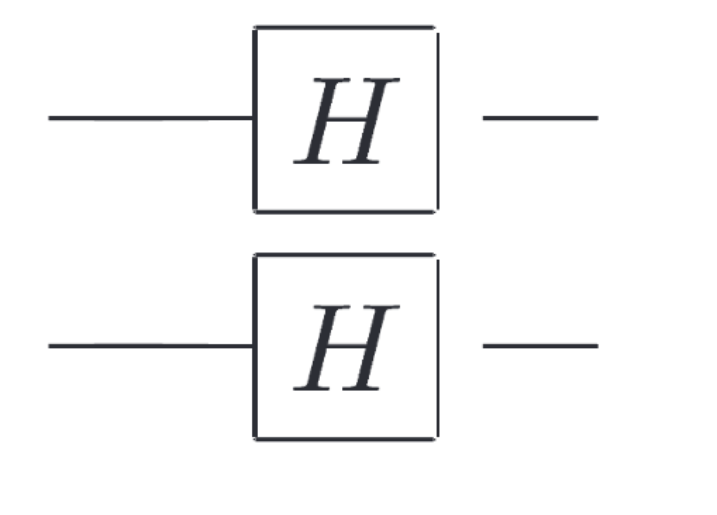
\includegraphics[width=0.6\textwidth]{Multyhadamard.png}
		\caption{اعمال تبدیل هادامارد $\operatorname{H} \otimes n$روی دو کیوبیت}
	\end{figure}
\end{center}

تبدیل هادامارد $\operatorname{H} \otimes 2$ روی دو بیت کوانتومی پیاده می‌شود. ارزیابی موازی کوانتومی یک تابع f(x) با ورودی n بیتی x و خروجی 1 بیتی، به روش زیر قابل پیاده‌سازی می‌باشد:

\begin{enumerate}
	\item ابتدا حالت $n + 1$ کیوبیت $\vert0\rangle^{\otimes n} \vert 0\rangle$ را آماده کنید،
	\item سپس تبدیل هادامارد را به $n$ کیوبیت اول و به دنبال آن مدار کوانتومی اعمال کنید.
	\item اعمال تابع $U_{f}$ به کیوبیت‌هایی که در حالت برهمنهی قرار دارند.
\end{enumerate}
درنهایت حالت زیر تولید ‌می‌شود:

\begin{center}
\begin{equation}
\frac{1}{\sqrt{2^n}} \sum_{x} \vert x \rangle \vert f (x)\rangle
\end{equation}
\end{center}


به طور کلی موازی‌سازی کوانتومی امکان ارزیابی همزمان همه مقادیر ممکن تابع f را فراهم می‌کند، حتی اگر ظاهراً فقط یک بار f را ارزیابی کرده باشیم. با این حال، این موازی‌سازی بلافاصله مفید نیست. 

در مثال تک کیوبیتی ما، اندازه‌گیری حالت فقط $\vert 0, f(0)\rangle$ یا $\vert 1, f(1)\rangle$ را می‌دهد! به طور مشابه، در حالت کلی، اندازه‌گیری حالت $\sum_{x} \vert x, f(x) \rangle$ فقط $ f (x)$ را برای یک مقدار $x$ خاص می‌دهد. البته یک کامپیوتر کلاسیک می‌تواند این کار را به راحتی انجام دهد! محاسبات کوانتومی برای مفید بودن به چیزی بیش از موازی‌سازی کوانتومی نیاز دارد؛ به توانایی استخراج اطلاعات مربوط به بیش از یک مقدار $f (x)$ از حالت‌های برهمنهی مانند $\sum _{x}\vert x, f(x) \rangle$ نیاز دارد. 
در بخش های بعدی به مثال‌های خواهیم پرداخت که این مسائل را حل کند.
\subsection{مدل محاسباتی استاندارد}
پیش از بررسی مدل کوئری،‌ مدل ساده و استاندارد محاسباتی را بررسی می‌کنیم. به تصویر زیر دقت کنید:

\begin{figure}[ht]
	\centering
	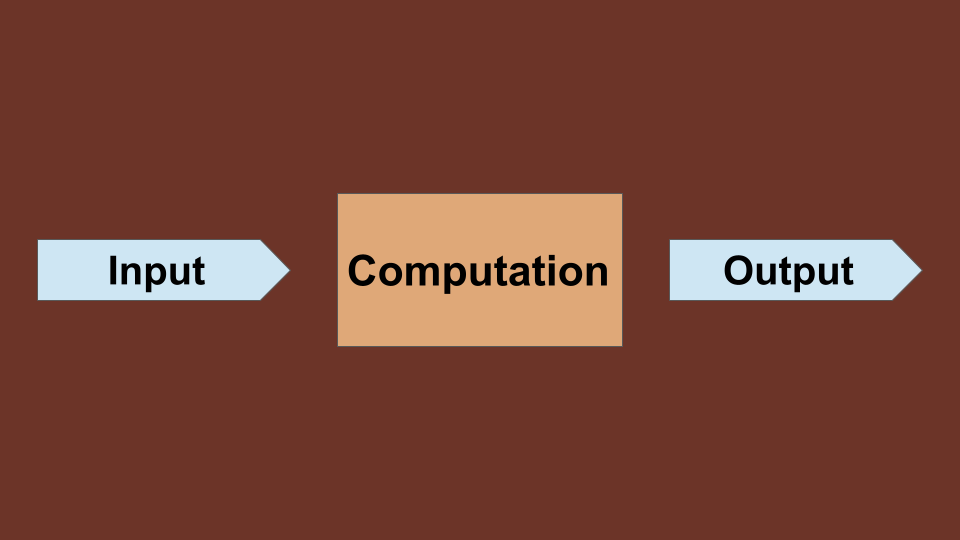
\includegraphics[width=0.8\textwidth]{standard computation model.png}
	\caption{یک واحد محاسباتی که مقادیری را به عنوان ورودی گرفته، پردازش کرده و سپس مقدار/مقادیر خروجی را ارائه کرده است.}
\end{figure}


در تصویر بالا یک نمود ساده از کامپیوتر‌های امروزی ارائه شده است. در دنیای واقعی مقدار ورودی می‌تواند از هر منبعی‌ تأمین شده باشد. با این وجود هدف ما بررسی منابع تولید ورودی نیست؛‌ بلکه هدف بررسی مقادیر ورودی (به صورت ایزوله) می‌باشد. می‌توان درنظر گرفت که ورودی داده شده و خروجی نهایی،‌هر دو در قالب یک رشته از اعداد باینری، ماتریس و یا هرقالب مدنظر کاربر باشند.

مهم‌ترین نکته درباره‌ی این واحد محاسباتی،‌ \textbf{در دسترس بودن کل مقادیر ورودی برای واحد پردازش} است. به عبارت دیگر\textbf{ واحد پردازش می‌تواند تمامی مقادیر ورودی را دریافت کرده و تشخیص} دهد. 

\section{مدل کوئری}
در مدل کوئری، داده‌های ورودی توسط یک تابع تولید می‌شوند. واحد محاسباتی دسترسی به تابع تولیدورودی دارد و می‌تواند برای دریافت داده‌های جدید،‌از تابع یاد شده،‌درخواست کند.

\begin{figure}[ht]
	\centering
	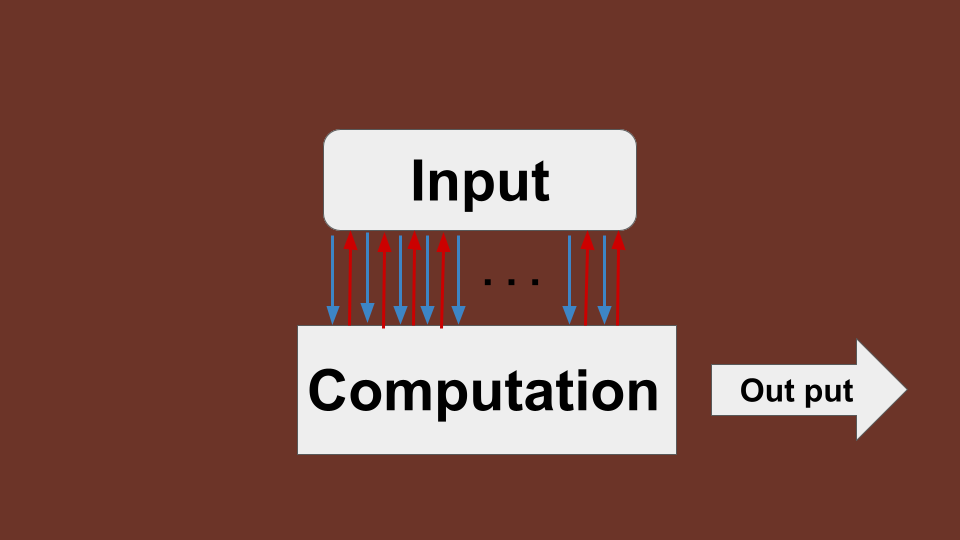
\includegraphics[width=0.8\textwidth]{Query computation model.png}
	\caption{شکل بالا نمود مدل محاسباتی‌کوئری است. واحد محاسباتی برای دریافت داده‌های جدید نیاز به درخواست از تابع ورودی دارد. خطوط قرمز و روبه‌بالا نشان از درخواست واحد محاسباتی و خطوط آبی روبه‌پایین نشان از پاسخ واحد ورودی می‌باشد.}
\end{figure}


در این مدل واحد محاسباتی دیگر داده‌ها را در قالب رشته‌ای از اطلاعات دردسترس ندارد؛ بلکه می‌تواند آن‌ها را از بخش تولید ورودی دریافت کند. در گاهی از مواقع به سیستم ورودی را اوراکل یا جعبه‌ی سیاه می‌نامند. تابع اوراکل\footnote{Oracle} یا جعبه‌ی سیاه\footnote{Black Box} یک سیستم است که ما به عنوان ناظر به سازوکار داخلی آن و  تمامی اطلاعات آن دسترسی نداریم و فقط می‌توانیم مقادیر مجاز را به آن داده و مقادیر خروجی را دریافت کنیم. 

تابع اوراکل به صورت زیر تعریف می‌شود:
\begin{center}
	\begin{equation}\label{key}
		\left\{
		\begin{array}{ll}
			f : \sum^n = \sum^m\\
			Which : m, n \in \mathbb{N}
		\end{array}
		\right.
	\end{equation}
\end{center}

ما در این نظریه کوئری‌ها را می‌شماریم و وضعیت آن‌‌ها را بررسی می‌کنیم.

\section{معرفی و پیاده سازی الگوریتم دوچ}

\subsection{مسئله‌ی دوچ}
الگوریتم دوچ\footnote{Deutsch algorithm} اولین و ساده‌ترین الگوریتم کوانتومی‌ است. این الگوریتم برای اولین بار در سال 1985 در مقاله‌ای مطرح شد؛ که توسط دیوید دوچ\footnote{\lr{David Deutsch}} نوشته شده‌‌بود. این الگوریتم نقطه‌ی شروعی برای اثبات برتری کامپیوترهای کوانتومی نسبت به کامپوترهای کلاسیک است.

مسئله‌ی دوچ یکی از ساده‌ترین مفاهیم ممکن را مطرح می‌کند. اگر یک تابع به فرم زیر تعریف شود: 
\begin{center}
	$f : \sum \rightarrow \sum$
\end{center}
هدف بررسی ثابت بودن یا متعادل\footnote{\lr{Constante or balanse.}} بودن تابع \lr{f} است. 
به‌طور کلی، درساده‌ترین حالت، می‌توان چهار وضعیت را برای تابع $f : \sum \rightarrow \sum$ درنظر گرفت:\\
\begin{figure}[ht]
	\centering
	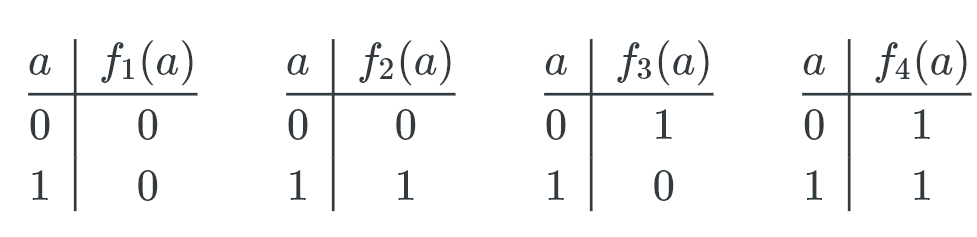
\includegraphics[width=0.8\textwidth]{Constantorbalanse.png}
	\caption{تمام حالات ممکن برای یک تابع ثابت و یک تابع متعادل}
\end{figure}\\
در شکل بالا توابع \lr{f 1} , \lr{f 4} توابع ثابت و توابع \lr{f 2} و \lr{f 3} توابع متعادل هستند.
\begin{center}
\begin{tabular}{|c|c|}
	\hline
	\multicolumn{2}{|c|}{مسئله‌ی دوچ} \\
	\hline
	$f : \sum \rightarrow \sum$ & ورودی \\
	\hline
	صفر اگر تابع ثابت بود؛ یک اگر تابع متعادل بود.  & خروجی \\
	\hline
\end{tabular}
\end{center}
در الگوریتم‌های کلاسیک برای حل این مسئله، حداقل دو حالت باید بررسی شود.
\subsection{الگوریتم دوچ}
% quantum computer scinse : read it for yourself
% https://www.youtube.com/watch?v=2wticzHE1vs&t=2014s
% page 32

حال به بررسی الگوریتم دوچ می‌پردازیم. الگوریتمی که مسئله‌ی دوچ را با یک مدار کوانتومی حل می‌کند:\\
\begin{center}
\begin{figure}[ht]
	\centering
	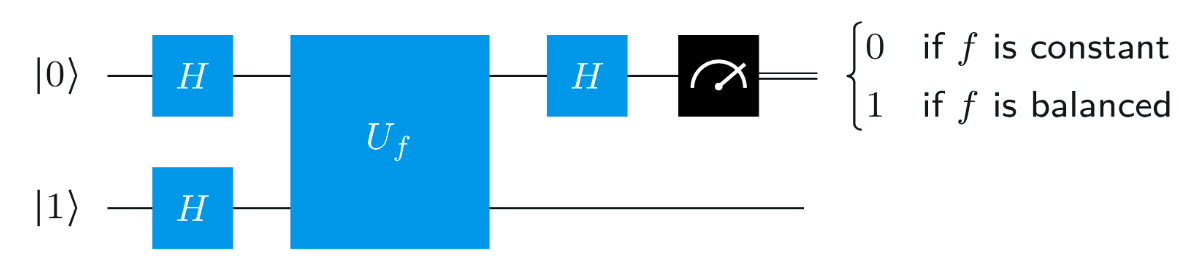
\includegraphics[width=0.8\textwidth]{Deutsch algorithm.png}
	\caption{}
\end{figure}
\end{center}


مدار زیر نشان می دهد که چگونه مدارهای کوانتومی می توانند با پیاده سازی الگوریتم دوچ از مدارهای کلاسیک پیشی بگیرند\footnote{ما در واقع یک نسخه ساده شده و بهبود یافته از الگوریتم اصلی را ارائه می دهیم.}. الگوریتم دوچ ترکیبی از موازی سازی کوانتومی با خاصیتی از مکانیک کوانتوم به نام تداخل\footnote{how interference is using in deutsch algorithm : Interference is used in the Deutsch algorithm to distinguish between constant and balanced functions. A constant function is a function that always returns the same value, regardless of its input. A balanced function is a function that returns 0 for half of its inputs and 1 for the other half.
	
	The Deutsch algorithm works by first preparing two qubits in a superposition of states. The first qubit is prepared in the state |+⟩, which is the equal superposition of $\vert 0 \rangle$ and $\vert 1 \rangle$. The second qubit is prepared in the state |ψ⟩, which is a superposition of the states $\vert 0 \rangle$ and $\vert 1 \rangle$ with opposite phases.
	
	The two qubits are then passed through a quantum circuit that includes a Hadamard gate and a CNOT gate. The Hadamard gate transforms |+⟩ into the superposition $\vert 0 \rangle$ + $\vert 1 \rangle$, and the CNOT gate copies the state of the first qubit to the second qubit.
	
	After the quantum circuit has been executed, the two qubits are measured. If the first qubit is measured to be $\vert 0 \rangle$, then the function f is constant. This is because the state |ψ⟩ is orthogonal to the state $\vert 0 \rangle$, so the interference between the two states will destructively interfere.
	
	If the first qubit is measured to be $\vert 1 \rangle$, then the function f is balanced. This is because the state |ψ⟩ is parallel to the state $\vert 1 \rangle$, so the interference between the two states will constructively interfere.
	
	The Deutsch algorithm is a simple example of how quantum interference can be used to solve a problem that is difficult to solve classically. In this case, the Deutsch algorithm can distinguish between constant and balanced functions in a single step, while a classical computer would need to take an exponential number of steps.} است.
مشابه قبل،‌ابتدا از گیت هادامارد برای آماده سازی اولین کیوبیت به عنوان برهمنهی $\frac{(\vert 0 \rangle + \vert 1 \rangle)}{\sqrt{2}}$استفاده کنیم، اما اکنون کیوبیت دوم y را با اعمال یک گیت هادامارد به حالت $\vert 1 \rangle$ به عنوان بهرهمنهی $\frac{(\vert 0 \rangle - \vert 1 \rangle)}{\sqrt{2}}$ آماده کنیم. به‌شکل زیر دقت کنید:



\begin{figure}[ht]
	\centering
	\includegraphics[width=0.8\textwidth]{Quantum circuit implementing Deutsch’s algorithm.png}
	\caption{پیاده‌سازی مدارکوانتومی‌ الگوریتم دوچ}
\end{figure}
حالت ورودی:\\
\begin{center}
	\begin{equation}\label{zero state deutsch}
		\vert\psi_{0}\rangle = \vert01\rangle
	\end{equation}
\end{center}

سیستم دو کیوبیتی تشکیل شده،‌ پس از اعمال اثر دو گیت هادامارد می‌دهد:\\

\begin{center}
	\begin{equation}\label{first psi1 deutsch algorithm}
		\left|\psi_1\right\rangle=\left[\frac{|0\rangle+|1\rangle}{\sqrt{2}}\right]\left[\frac{|0\rangle-|1\rangle}{\sqrt{2}}\right]
	\end{equation}
\end{center}
با کمی تأمل می‌توان دریافت که اگر $U_{f}$ را به حالت $\vert x \rangle (\vert 0 \rangle - \vert 1 \rangle)/\sqrt{2}$ اعمال کنیم، سپس به حالت $(-1)^{f(x)}\vert x \rangle(\vert 0 \rangle - \vert 1 \rangle)/\sqrt{2}$ می رسیم. بنابرین اعمال $U_{f}$ به $\vert \Psi_{1} \rangle$ ما را با یکی از دو امکان زیر مواجه می کند:
\begin{center}
	\begin{equation}\label{first psi2 deutsch algorithm}
	\left|\psi_2\right\rangle= \begin{cases} \pm\left[\frac{|0\rangle+|1\rangle}{\sqrt{2}}\right]\left[\frac{|0\rangle-|1\rangle}{\sqrt{2}}\right] & \text { if } f(0)=f(1) \\ \pm\left[\frac{|0\rangle-|1\rangle}{\sqrt{2}}\right]\left[\frac{|0\rangle-|1\rangle}{\sqrt{2}}\right] & \text { if } f(0) \neq f(1) \end{cases}
\end{equation}
\end{center}
با اعمال آخرین گیت هادامارد روی کیوبیت اول به حالت زیر خواهیم رسید:
\begin{center}
	\begin{equation}\label{first psi3 deutsch algorithm}
	\left|\psi_3\right\rangle= \begin{cases} \pm|0\rangle\left[\frac{|0\rangle-|1\rangle}{\sqrt{2}}\right] & \text { if } f(0)=f(1) \\ \pm|1\rangle\left[\frac{|0\rangle-|1\rangle}{\sqrt{2}}\right] & \text { if } f(0) \neq f(1) \end{cases}
	\end{equation}
\end{center}
با درنظر گرفتن شرایط زیر می‌توان $\vert\psi_{3}\rangle$ را به شکل زیر بازنویسی کرد:
\begin{center}
\begin{equation}\label{constantorbalanse}
	\begin{aligned}
		\left\{
		\begin{aligned}
			f(0) &= f(1) 
			\implies \qquad f(0) \oplus f(1) &= 0\\
			f(0) &\neq f(1) 
			\implies \qquad f(0) \oplus f(1) &= 1
		\end{aligned}
		\right.
	\end{aligned}
\end{equation}
\end{center}
از این رو:
\begin{center}
	\begin{equation}\label{psi3 deutsch algorithm}
	\left|\psi_3\right\rangle= \pm|f(0) \oplus f(1)\rangle\left[\frac{|0\rangle-|1\rangle}{\sqrt{2}}\right]	
	\end{equation}
\end{center}
بنابراین با اندازه گیری کیوبیت اول می توانیم $f(0) \oplus f(1)$ را تعیین کنیم. واقعاً جالب است! مدار کوانتومی به ما توانایی تعیین یک ویژگی کلی از $f(x)$، یعنی$ f(0)\oplus f(1)$ را داده است، با استفاده از تنها یک ارزیابی از $f(x)$!این سریعتر از آن چیزی است که با یک دستگاه کلاسیک امکان‌پذیر است،یک دستگاه کلاسیک حداقل به دو ارزیابی نیاز دارد.
این مثال تفاوت بین موازی‌سازی کوانتومی و الگوریتم‌های تصادفی کلاسیک را برجسته می‌کند. به سادگی، ممکن است تصور شود که حالت $\vert0\rangle \vert f(0) \rangle + \vert1\rangle \vert f(1) \rangle$ مطابقت نزدیکی با یک رایانه کلاسیک تصادفی دارد که هرکدام از حالات $ f (0)$ یا$ f (1) $ با احتمال $1/2$ اندازه‌گیری می‌کند.
تفاوت این است که در یک رایانه کلاسیک این دو گزینه همیشه یکدیگر را حذف می‌کنند. در یک رایانه کوانتومی، امکان دارد که دو گزینه با یکدیگر تداخل داشته باشند تا برخی از خواص کلی تابع $f$ را با استفاده از چیزی شبیه به گیت هادامارد برای بازترکیب گزینه‌های مختلف، مانند آنچه در الگوریتم دوچ انجام شد، به دست آورند.
اساس طراحی بسیاری از الگوریتم‌های کوانتومی این است که یک انتخاب هوشمندانه از تابع و تبدیل نهایی اجازه می‌دهد تا اطلاعات جهانی مفیدی در مورد تابع تعیین شود - اطلاعاتی که نمی‌توان به سرعت در یک رایانه کلاسیک به دست آورد.


% implimentation : https://learn.qiskit.org/course/ch-algorithms/deutsch-jozsa-algorithm

\subsection{پیاده‌سازی الگوریتم دوچ در کیس کیت}

ابتدا کتابخانه‌های مورد نیاز را فراخوانی می‌کنیم:
\begin{tcolorbox}[width=13cm, colback=gray9, boxsep=10pt, halign=center]
\begin{Verbatim}[commandchars=\\\{\}]
\PY{k+kn}{from} \PY{n+nn}{qiskit} \PY{k+kn}{import} \PY{o}{*}
\PY{k+kn}{from} \PY{n+nn}{qiskit}\PY{n+nn}{.}\PY{n+nn}{tools}\PY{n+nn}{.}\PY{n+nn}{visualization} \PY{k+kn}{import} \PY{n}{plot\PYZus{}histogram}
\PY{o}{\PYZpc{}}\PY{k}{matplotlib} inline
\end{Verbatim}
\end{tcolorbox}

یک مدار کوانتومی با دو کیوبیت و یک بیت کلاسیک ایجاد می‌کنیم؛ این الگوریتم با یک بیت کلاسیک نیز قابل اجراست. کیوبیت‌ اول برای بررسی تابع ایجاد شده و کیوبیت دوم برای کنترل بهتر شرایط ایجاد شده است:
\begin{tcolorbox}[width=13cm, colback=gray9, boxsep=10pt, halign=center]
\begin{Verbatim}[commandchars=\\\{\}]
\PY{n}{circuit} \PY{o}{=} \PY{n}{QuantumCircuit}\PY{p}{(}\PY{l+m+mi}{2}\PY{p}{,}\PY{l+m+mi}{1}\PY{p}{)}
\end{Verbatim}
\end{tcolorbox}
به اولین کیوبیت یک گیت هادامارد اثر می‌دهیم. سپس بر دومین کیوبیت،‌ به ترتیب یک گیت ایکس پائولی و یک گیت هادامارد اثر می‌دهیم:
\begin{tcolorbox}[width=13cm, colback=gray9, boxsep=10pt, halign=center]
\begin{Verbatim}[commandchars=\\\{\}]
\PY{n}{circuit}\PY{o}{.}\PY{n}{h}\PY{p}{(}\PY{l+m+mi}{0}\PY{p}{)}
\PY{n}{circuit}\PY{o}{.}\PY{n}{x}\PY{p}{(}\PY{l+m+mi}{1}\PY{p}{)}
\PY{n}{circuit}\PY{o}{.}\PY{n}{h}\PY{p}{(}\PY{l+m+mi}{1}\PY{p}{)}
\PY{n}{circuit}\PY{o}{.}\PY{n}{barrier}\PY{p}{(}\PY{p}{)}
\PY{n}{circuit}\PY{o}{.}\PY{n}{draw}\PY{p}{(}\PY{n}{output}\PY{o}{=}\PY{l+s+s1}{\PYZsq{}}\PY{l+s+s1}{mpl}\PY{l+s+s1}{\PYZsq{}}\PY{p}{)}
\end{Verbatim}
\end{tcolorbox}

\begin{center}
\begin{figure}[h]
	\centering
	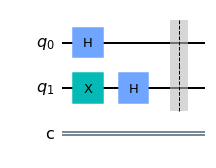
\includegraphics[width=0.5\linewidth]{output_2_0.png}
	\caption{آماده‌سازی دو کیوبیت}
\end{figure}
\end{center}
حال یک گیت \lr{CNOT} با هدف قرار دادن کیوبیت دوم به مدار اعمال می‌کنیم. سپس گیت هادامارد را بر اولین کیوبیت اعمال ‌می‌کنیم؛ چرا که قصد اندازه‌گیری این کیوبیت را داریم:
\begin{tcolorbox}[width=13cm, colback=gray9, boxsep=10pt, halign=center]
\begin{Verbatim}[commandchars=\\\{\}]
\PY{n}{circuit}\PY{o}{.}\PY{n}{cx}\PY{p}{(}\PY{l+m+mi}{0}\PY{p}{,}\PY{l+m+mi}{1}\PY{p}{)}
\PY{n}{circuit}\PY{o}{.}\PY{n}{barrier}\PY{p}{(}\PY{p}{)}
\PY{n}{circuit}\PY{o}{.}\PY{n}{h}\PY{p}{(}\PY{l+m+mi}{0}\PY{p}{)}
\PY{n}{circuit}\PY{o}{.}\PY{n}{barrier}\PY{p}{(}\PY{p}{)}
\PY{n}{circuit}\PY{o}{.}\PY{n}{draw}\PY{p}{(}\PY{n}{output}\PY{o}{=}\PY{l+s+s1}{\PYZsq{}}\PY{l+s+s1}{mpl}\PY{l+s+s1}{\PYZsq{}}\PY{p}{)}
\end{Verbatim}
\end{tcolorbox}

\begin{center}
\begin{figure}[h]
\centering
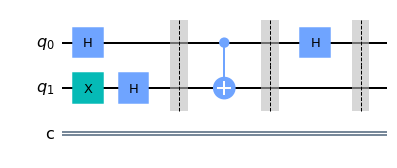
\includegraphics[width=0.8\linewidth]{output_3_0.png}
\caption{وضعیت مدار پس از اعمال اوراکل بر کیوبیت ها}
\end{figure}
\end{center}
حال اندازه‌گیری را انجام می‌دهیم:
\begin{tcolorbox}[width=13cm, colback=gray9, boxsep=10pt, halign=center]
\begin{Verbatim}[commandchars=\\\{\}]
\PY{n}{circuit}\PY{o}{.}\PY{n}{measure}\PY{p}{(}\PY{l+m+mi}{0}\PY{p}{,}\PY{l+m+mi}{0}\PY{p}{)}
\end{Verbatim}
\end{tcolorbox}
\begin{tcolorbox}[width=13cm, colback=gray9, boxsep=10pt, halign=center]
\begin{Verbatim}[commandchars=\\\{\}]
<qiskit.circuit.instructionset.InstructionSet at 0x7fb3a83c1c70>
\end{Verbatim}
\end{tcolorbox}

\begin{tcolorbox}[width=13cm, colback=gray9, boxsep=10pt, halign=center]
\begin{Verbatim}[commandchars=\\\{\}]
\PY{n}{circuit}\PY{o}{.}\PY{n}{draw}\PY{p}{(}\PY{n}{output}\PY{o}{=}\PY{l+s+s1}{\PYZsq{}}\PY{l+s+s1}{mpl}\PY{l+s+s1}{\PYZsq{}}\PY{p}{)}
\end{Verbatim}
\end{tcolorbox}

\begin{center}
\begin{figure}[h]
\centering
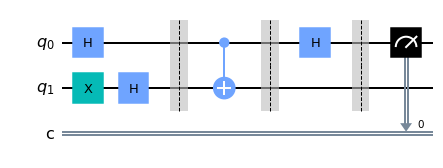
\includegraphics[width=0.8\linewidth]{output_5_0.png}
\caption{مدار کوانتومی کامل که روی شبیه‌ساز کلاسیک پیاده‌سازی شده‌است.}
\end{figure}
\end{center}

حال این کد را به شبیه‌ساز کلاسیک \lr{IBM} منتقل می‌کنیم:
\begin{tcolorbox}[width=13cm, colback=gray9, boxsep=10pt, halign=center]
\begin{Verbatim}[commandchars=\\\{\}]
\PY{n}{backend} \PY{o}{=} \PY{n}{Aer}\PY{o}{.}\PY{n}{get\PYZus{}backend}\PY{p}{(}\PY{l+s+s1}{\PYZsq{}}\PY{l+s+s1}{qasm\PYZus{}simulator}\PY{l+s+s1}{\PYZsq{}}\PY{p}{)}
\PY{n}{result} \PY{o}{=} \PY{n}{execute}\PY{p}{(}\PY{n}{circuit}\PY{p}{,} \PY{n}{backend}\PY{o}{=}\PY{n}{backend}\PY{p}{,} \PY{n}{shots}\PY{o}{=}\PY{l+m+mi}{1024}\PY{p}{)}\PY{o}{.}\PY{n}{result}\PY{p}{(}\PY{p}{)}
\PY{n}{counts} \PY{o}{=} \PY{n}{result}\PY{o}{.}\PY{n}{get\PYZus{}counts}\PY{p}{(}\PY{n}{circuit}\PY{p}{)}

\PY{n}{plot\PYZus{}histogram}\PY{p}{(}\PY{p}{[}\PY{n}{counts}\PY{p}{]}\PY{p}{)}
\end{Verbatim}
\end{tcolorbox}

\begin{center}
\begin{figure}[h]
\centering
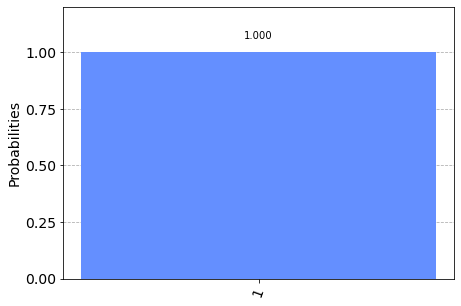
\includegraphics[width=0.6\linewidth]{output_6_0.png}
\caption{خروجی شبیه‌سازی برابر با یک شده است. طبق فرمول \ref{constantorbalanse} این تابع یک تابع متعادل است.}
\end{figure}
\end{center}
به ازای تمامی شات‌ها(تعداد دفعات تکرار آزمایش) به مقدار یک دست یافتیم؛ این به معنای متعادل بودن تابع است. حال وقت آن رسیده ‌‌که با کامپیوتر کوانتومی حقیقی کار کنیم. همانطور که در بخش ~\ref{sec:Qiskit} گفته شد؛ می‌بایست با حساب کاربری خود به این کامپیوتر کوانتومی وصل شویم:

\begin{latin}
\begin{tcolorbox}[width=13cm, colback=gray9, boxsep=10pt, halign=center]
\begin{Verbatim}[commandchars=\\\{\}]
\PY{c+c1}{\PYZsh{}Real Quantum Computer}
\PY{n}{IBMQ}\PY{o}{.}\PY{n}{load\PYZus{}account}\PY{p}{(}\PY{p}{)}
\end{Verbatim}
\end{tcolorbox}
\end{latin}

\begin{tcolorbox}[width=14cm, colback=gray9, boxsep=10pt, halign=center]
\begin{Verbatim}[commandchars=\\\{\}]
<AccountProvider for IBMQ(hub='ibm-q', group='open', project='main')>
\end{Verbatim}
\end{tcolorbox}
حال لیست کامپیوتر‌های کوانتومی که بیشترین منابع را در اختیار دارند را استخراج می‌کنیم:

\begin{tcolorbox}[width=13cm, colback=gray9, boxsep=10pt, halign=center]
\begin{Verbatim}[commandchars=\\\{\}]
\PY{n}{provider} \PY{o}{=} \PY{n}{IBMQ}\PY{o}{.}\PY{n}{get\PYZus{}provider}\PY{p}{(}\PY{l+s+s2}{\PYZdq{}}\PY{l+s+s2}{ibm\PYZhy{}q}\PY{l+s+s2}{\PYZdq{}}\PY{p}{)}

\PY{k}{for} \PY{n}{backend} \PY{o+ow}{in} \PY{n}{provider}\PY{o}{.}\PY{n}{backends}\PY{p}{(}\PY{p}{)}\PY{p}{:}
\PY{k}{try}\PY{p}{:}
\PY{n}{qubit\PYZus{}count} \PY{o}{=} \PY{n+nb}{len}\PY{p}{(}\PY{n}{backend}\PY{o}{.}\PY{n}{properties}\PY{p}{(}\PY{p}{)}\PY{o}{.}\PY{n}{qubits}\PY{p}{)}
\PY{k}{except}\PY{p}{:}
\PY{n}{qubit\PYZus{}count} \PY{o}{=} \PY{l+s+s2}{\PYZdq{}}\PY{l+s+s2}{simulated}\PY{l+s+s2}{\PYZdq{}}
\PY{n+nb}{print}\PY{p}{(}\PY{l+s+sa}{f}\PY{l+s+s2}{\PYZdq{}}\PY{l+s+si}{\PYZob{}}\PY{n}{backend}\PY{o}{.}\PY{n}{name}\PY{p}{(}\PY{p}{)}\PY{l+s+si}{\PYZcb{}}\PY{l+s+s2}{ : }
	\PY{l+s+si}{\PYZob{}}\PY{n}{backend}\PY{o}{.}\PY{n}{status}\PY{p}{(}\PY{p}{)}\PY{o}{.}\PY{n}{pending\PYZus{}jobs}\PY{l+s+si}{\PYZcb{}}\PY{l+s+s2}{ \PYZam{} }\PY{l+s+si}{\PYZob{}}\PY{n}{qubit\PYZus{}count}\PY{l+s+si}{\PYZcb{}}\PY{l+s+s2}{ qubits}\PY{l+s+s2}{\PYZdq{}}\PY{p}{)}
\end{Verbatim}
\end{tcolorbox}
لیست وضعیت کامپیوترهای‌کوانتومی در حین اجرای این کد به شرح زیر بوده‌است:
\begin{tcolorbox}[width=13cm, colback=gray9, boxsep=10pt, halign=center]
\begin{Verbatim}[commandchars=\\\{\}]
ibmq\_qasm\_simulator : 3 \& simulated qubits
ibmqx2 : 12 \& 5 qubits
ibmq\_16\_melbourne : 411 \& 15 qubits
ibmq\_armonk : 48 \& 1 qubits
ibmq\_athens : 7 \& 5 qubits
ibmq\_santiago : 13 \& 5 qubits
ibmq\_lima : 12 \& 5 qubits
ibmq\_belem : 5 \& 5 qubits
ibmq\_quito : 4 \& 5 qubits
simulator\_statevector : 4 \& simulated qubits
simulator\_mps : 3 \& simulated qubits
simulator\_extended\_stabilizer : 3 \& simulated qubits
simulator\_stabilizer : 3 \& simulated qubits
ibmq\_manila : 15 \& 5 qubits
\end{Verbatim}
\end{tcolorbox}
از کامپیوتر \lr{ibqm-belem} استفاده می‌کنیم:
\begin{tcolorbox}[width=13cm, colback=gray9, boxsep=10pt, halign=center]
\begin{Verbatim}[commandchars=\\\{\}]
\PY{n}{quantum\PYZus{}computer} \PY{o}{=} \PY{n}{provider}\PY{o}{.}\PY{n}{get\PYZus{}backend}\PY{p}{(}\PY{l+s+s1}{\PYZsq{}}\PY{l+s+s1}{ibmq\PYZus{}belem}\PY{l+s+s1}{\PYZsq{}}\PY{p}{)}
\end{Verbatim}
\end{tcolorbox}

\begin{tcolorbox}[width=15.5cm, colback=gray9, boxsep=10pt, halign=center]
\begin{Verbatim}[commandchars=\\\{\}]
\PY{n}{quantum\PYZus{}result} \PY{o}{=} \PY{n}{execute}\PY{p}{(}\PY{n}{circuit}\PY{p}{,} \PY{n}{backend}\PY{o}{=}\PY{n}{quantum\PYZus{}computer}\PY{p}{,}\PY{n}{shots}\PY{o}{=}\PY{l+m+mi}{1024}\PY{p}{)}\PY{o}{.}\PY{n}{result}\PY{p}{(}\PY{p}{)}
\end{Verbatim}
\end{tcolorbox}

حال مقادیر محاسبه شده را به تصویر می‌کشیم:
\begin{tcolorbox}[width=13cm, colback=gray9, boxsep=10pt, halign=center]
\begin{Verbatim}[commandchars=\\\{\}]
\PY{n}{quantum\PYZus{}counts} \PY{o}{=} \PY{n}{quantum\PYZus{}result}\PY{o}{.}\PY{n}{get\PYZus{}counts}\PY{p}{(}\PY{n}{circuit}\PY{p}{)}
\PY{n}{plot\PYZus{}histogram}\PY{p}{(}\PY{p}{[}\PY{n}{quantum\PYZus{}counts}\PY{p}{]}\PY{p}{)}
\end{Verbatim}
\end{tcolorbox}
\begin{center}
\begin{figure}[h]
\centering
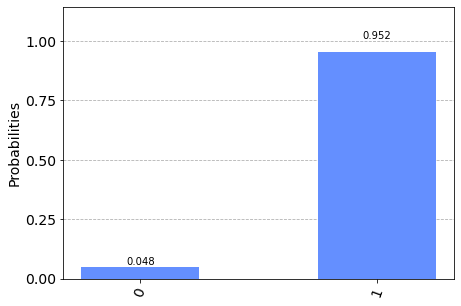
\includegraphics[width=0.5\linewidth]{output_13_0.png}
\caption{مقادیر محاسبه‌شده باکمک کامپیوتر کوانتومی}
\end{figure}
\end{center}
همانطور که مشاهده می‌شود؛ در کل شات‌های پیاده‌سازی مدار ایجاد شده، عدد یک در اغلب موارد به‌عنوان حاصل اعلام شده است. مابقی نتایح به عنوان نویز دسته‌بندی می‌شوند.

\chapter{شبیه‌سازی پدیده‌های کوانتومی}
در این بخش قصد داریم به بررسی پروتکل‌های ابتدایی در نظریه‌ی اطلاعات کوانتومی بپردازیم. تمامی این پروتکل‌ها به تعداد کمی کیوبیت نیاز دارند؛ و در آزمایشگاه به صورت تجربی پیاده‌سازی شده‌اند. 
\section{حالات بل}
به مدار نمایش داده شده در شکل زیر دقت کنید:

این مدار دارای یک گیت هادامارد و سپس CNOT است و چهار حالت پایه محاسباتی را مطابق جدول داده شده تبدیل می کند. به عنوان مثال:
 گیت هادامارد ورودی $\vert 00 \rangle$ را به حالت  $\frac{(\vert 0 \rangle + \vert 1 \rangle)}{\sqrt{2}}$ انتقال می‌دهد و سپس CNOT حالت خروجی $\frac{(\vert 00 \rangle + \vert 11 \rangle)}{\sqrt{2}}$ را آماده می‌کند.\\ 
 
 بار دیگر مراحل را مرور می‌کنیم:\\
  ابتدا اعمال تبدیل هادامارد حالت کیوبیت بالایی را به یک برهمنهی کوانتومی منتقل می‌کند. این برهمنهی ایجاد شده،‌ به عنوان کیوبیت کنترل به CNOT عمل می کند و حالت کیوبیت هدف تنها زمانی معکوس می شود که حالت کیوبیت کنترل 1 باشد.\\
  
  
حالت خروجی را می‌توان به شکل زیر نمایش داد:\\

\begin{equation}
	%\begin{align*}
	\begin{split}
		\ket{\beta_{00}} &= \frac{\ket{00} + \ket{11}}{\sqrt{2}} \\
		\ket{\beta_{01}} &= \frac{\ket{01} + \ket{10}}{\sqrt{2}} \\
		\ket{\beta_{10}} &= \frac{\ket{00} - \ket{11}}{\sqrt{2}} \\
		\ket{\beta_{11}} &= \frac{\ket{01} - \ket{10}}{\sqrt{2}}
	\end{split}	
	%\end{align*}
\end{equation}

 از حالت‌های بالا به عنوان حالات بل یا حالات EPR یاد‌می‌کنیم.
  
  
خصوصیات حالات $\vert \beta_{00} \rangle, \vert \beta_{01} \rangle, \vert \beta_{10} \rangle, \vert \beta_{11} \rangle,$از طریق فرمول زیر بهتر درک خواهند شد:
\begin{equation}\label{Bell formula}
	\ket{\beta_{ay}} = \frac{\ket{0, y} + (-1)^{y} \ket{1, \bar{y}}}{\sqrt{2}}
\end{equation}

منظور از این جمله چیه؟؟
where ¯y is the negation of y.




 
\begin{figure}[h]
	\centering
	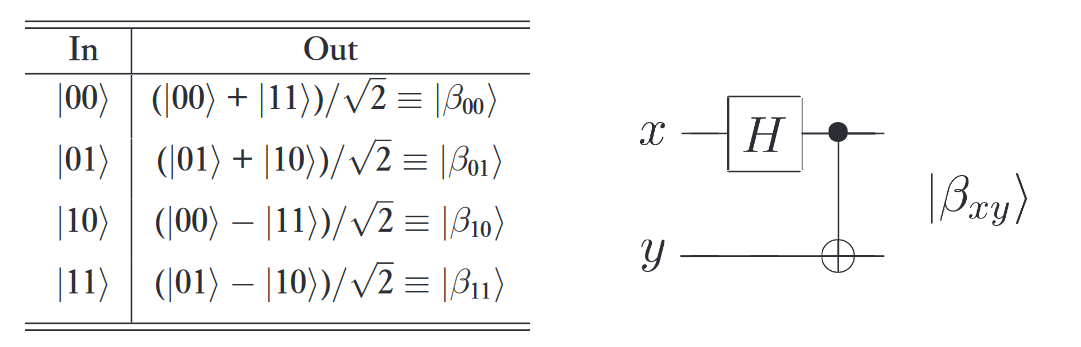
\includegraphics[width=0.8\textwidth]{Bell_state.png}
	\caption{مدار کوانتومی بل به‌همراه ورودی و خروجی آن}
\end{figure}

\section{درهمتنیدگی}
در حوزه فیزیک کوانتومی، یکی از گیج کننده ترین پدیده هایی که همچنان توجه دانشمندان و فیلسوفان را به خود جذب می کند، «درهم تنیدگی» است. این مفهوم درک متعارف ما از واقعیت را به چالش می‌کشد و باعث بحث‌ها، آزمایش‌ها و تحقیقات فلسفی بی‌شماری شده است.\\
درهم تنیدگی به ارتباط فوق‌العاده‌ای اطلاق می‌شود که می‌تواند بین دو یا چند ذره، بدون توجه به فاصله‌ای که آنها را از هم، وجود داشته باشد. هنگامی که ذرات در هم می‌پیچند، ویژگی‌های آن‌ها مانند اسپین، تکانه و قطبش به گونه‌ای به هم مرتبط می‌شوند که تغییر حالت یک ذره بدون توجه به فضای فیزیکی بین آنها، فوراً بر وضعیت ذره دیگر تأثیر می‌گذارد. به نظر می‌رسد این ارتباط آنی با مفاهیم کلاسیک علت و معلول مخالفت می‌کند.\\

یکی از مشهورترین آزمایش‌های فکری که درهم تنیدگی را نشان می‌دهد، پارادوکس انیشتین-پودولسکی-روزن (EPR) است. در این سناریو، دو ذره درهم تنیده که اغلب به آنها «آلیس» و «باب» گفته می شود، جدا شده و به مکان های مختلف فرستاده می شوند. وقتی اندازه‌گیری روی یک ذره انجام می‌شود، حالت آن فوراً مشخص می‌شود و باعث می‌شود وضعیت ذره دیگر نیز مشخص شود، این تغییر حالت از راه دور حتی اگر دو ذره‌ی درهم‌تنیده سال‌های نوری از هم فاصله داشته باشند؛ رخ خواهد داد. این نقض آشکار محدودیت سرعت نور، درک ما از نحوه انتقال اطلاعات را به چالش کشیده است.\\

درهم تنیدگی فقط یک مفهوم نظری نیست. به طور تجربی از طریق آزمایش های مختلف مشاهده و تأیید شده است. یکی از مهم‌ترین آزمایش‌هایی که درهم تنیدگی را به صورت تجربی نشان می‌دهد، آزمون بل است.
این آزمایش نقض نابرابری‌های بل را آزمایش می‌کند. وقتی اندازه‌گیری‌های ذرات درهم تنیده این نابرابری‌ها را نقض می‌کند، نشان می‌دهد که رفتار آنها توسط فیزیک کلاسیک قابل توضیح نیست و در عوض به واقعیت درهم‌تنیدگی کوانتومی اشاره می‌کند.\\

پیامدهای درهم تنیدگی عمیق و پیچیده است و فراتر از محدوده آزمایشگاه های فیزیک است. محققان همواره در حال بررسی کاربردهای بالقوه درهم تنیدگی در زمینه هایی مانند محاسبات کوانتومی و رمزنگاری کوانتومی هستند. توانایی درهم تنیدگی برای فعال کردن کیوبیت‌ها (بیت‌های کوانتومی) برای وجود همزمان در چندین حالت، این پتانسیل ایجاد تحولات شگرفی در رمزنگاری کوانتومی و محاسبات کوانتومی دارد و به راه‌حل‌هایی منجر شود که قبلا غیرممکن تلقی می‌شدند.\\

در نتیجه، از درهم تنیدگی به عنوان یکی از جذاب ترین و گیج کننده ترین پدیده ها در قلمرو فیزیک کوانتومی یاد‌می‌شود. ارتباط اسرارآمیز آن بین ذرات، شهود کلاسیک را به چالش می کشد و همچنان مرزهای درک ما از جهان را پیش می برد. همانطور که دانشمندان عمیق تر به پیچیدگی های درهم تنیدگی و کاربردهای بالقوه آن می پردازند.

\section{دوربری}
دوربری کوانتومی تکنیکی برای جابجایی حالات کوانتومی به نقاط دیگر است. در اینجا نحوه عملکرد دوربری کوانتومی آمده است:

 آلیس و باب مدت ها پیش با هم آشنا شدند اما اکنون دور از هم زندگی می کنند. در حالی که آنها با هم یک جفت EPR تولید کردند، هر کدام یک کیوبیت از جفت EPR را در هنگام جدا شدن می‌گرفتند. سالها بعد، باب مخفی است، و ماموریت آلیس، در صورتی که آن را بپذیرد، تحویل یک کیوبیت $\vert \Psi \rangle$ به باب است. او وضعیت  و خصوصیات کیوبیت را نمی داند و علاوه بر این فقط می تواند اطلاعات کلاسیک را برای باب ارسال کند. آیا آلیس باید این مأموریت را بپذیرد؟\\


درظاهر، تمام شرایط علیه آلیس است. او وضعیت $\vert \Psi \rangle$ کیوبیتی را که باید برای باب بفرستد نمی داند، و طبق قوانین مکانیک کوانتومی، او حق تعیین وضعیت $\vert \Psi \rangle$ را ندارد؛‌زیرا فقط یک نسخه از جفت کیوبیت را در اختیار دارد. به علاوه، حتی اگر او حالت $\vert \Psi \rangle$ را می دانست، توصیف دقیق آن به مقدار نامحدودی از اطلاعات کلاسیک نیاز دارد، زیرا $\vert \Psi \rangle$ مقادیری را در یک فضای پیوسته می گیرد.

بنابراین حتی اگر او $\vert \Psi \rangle$ را می دانست، برای آلیس تا ابد طول می کشید تا وضعیت را برای باب توصیف کند. دوربری کوانتومی راهی برای استفاده از جفت EPR درهم تنیده به منظور ارسال $\vert \Psi \rangle$ به باب، تنها با سربار کوچکی از ارتباطات کلاسیک است. این مسأله وضعیت را برای آلیس تغییر می‌دهد.

به طور کلی، مراحل حل به شرح زیر است: آلیس با کیوبیت $\vert \Psi \rangle$ با یک کیوبیت خود از جفت EPR، و سپس دو کیوبیت در اختیارش را اندازه گیری می کند و یکی از چهار نتیجه کلاسیک ممکن
، 00، 01، 10، 11 را بدست می‌آورد. درنهایت او این اطلاعات را به باب ارسال می‌کند.


 بسته به پیام کلاسیک آلیس، باب یکی از چهار عملگر جدول زیر را روی کیوبیت $EPR$ خود اعمال می‌کند.
 به طرز شگفت انگیزی، با انجام این کار او می تواند حالت اولیه را بازیابی کند $\vert \Psi \rangle$! مدار کوانتومی نشان داده شده در شکل زیر توصیف دقیق تری از دوربری کوانتومی ارائه می دهد.
دوربری حالتی که باید از راه دور منتقل شود عبارت است از $\vert \Psi \rangle = \alpha \vert 0 \rangle + \beta \vert 1 \rangle$ که $\alpha$ و $\beta$ ناشناخته هستند.

\begin{center}
	\begin{equation}\label{psi before spooky action}
		\left.\left|\psi_0\right\rangle=\vert \psi\rangle \vert \beta_{00}\right\rangle
	\end{equation}
\end{center}


\begin{figure}[h]
\centering
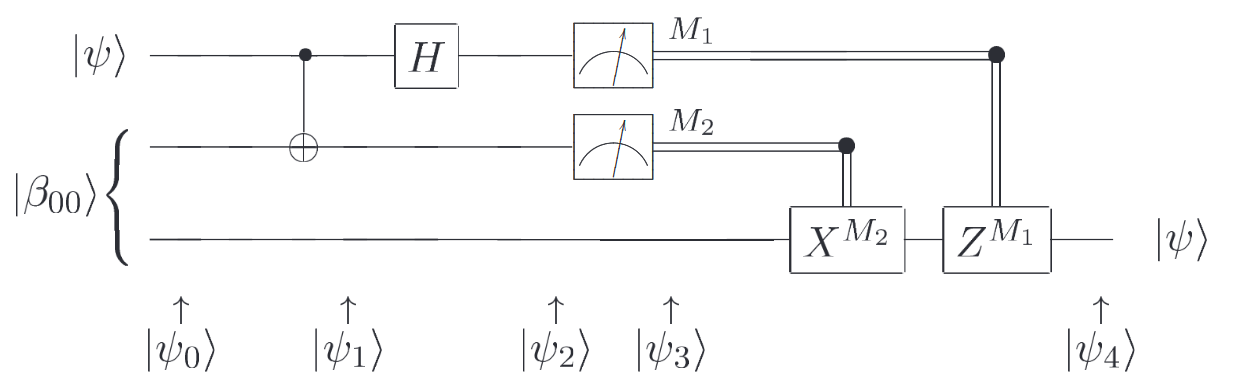
\includegraphics[width=6in]{spooky action.png}
\caption{مدار کوانتومی برای انتقال یک کیوبیت دو خط بالا نشان دهنده سیستم آلیس هستند، در حالی که خط پایین نشان دهنده سیستم آلیس است		خط سیستم باب است. مترها اندازه گیری را نشان می دهند و خطوط دوتایی که از آنها بیرون می آیند دارای حالت کلاسیک هستند
		بیت ها (به یاد بیاورید که خطوط منفرد نشان دهنده کیوبیت هستند)}
\end{figure}

\begin{center}
	\begin{equation}\label{wide version spooky psi}
		=\frac{1}{\sqrt{2}}[\alpha|0\rangle(|00\rangle+|11\rangle)+\beta|1\rangle(|00\rangle+|11\rangle)]
	\end{equation}
\end{center}

جایی که ما از این قاعده استفاده می کنیم که دو کیوبیت اول (در سمت چپ) متعلق به آلیس هستند و
کیوبیت سوم متعلق به باب است. همانطور که قبلا توضیح دادیم ، کیوبیت دوم آلیس و کیوبیت باب
در یک حالت EPR شروع می شوند. آلیس یک گیت $CNOT$ را روی کیوبیت‌های خود اثر می‌دهد. از این رو:


\begin{center}
	\begin{equation}\label{Teleport psi1}
		\left|\psi_1\right\rangle=\frac{1}{\sqrt{2}}[\alpha|0\rangle(|00\rangle+|11\rangle)+\beta|1\rangle(|10\rangle+|01\rangle)]
	\end{equation}
\end{center}

سپس گیت هادامارد را روی اولین کیوبیت اثر می‌دهد و به دست می آورد:

\begin{center}
	\begin{equation}\label{Teleport psi2}
		\left|\psi_2\right\rangle=\frac{1}{2}[\alpha(|0\rangle+|1\rangle)(|00\rangle+|11\rangle)+\beta(|0\rangle-|1\rangle)(|10\rangle+|01\rangle)]
	\end{equation}
\end{center}

این حالت را می توان به روش زیر بازنویسی کرد، به سادگی با گروه بندی مجدد عبارات:

\begin{center}
	\begin{equation}\label{Teleport psi2 rewrite}
		\begin{aligned}
			\left|\psi_2\right\rangle= & \frac{1}{2}[|00\rangle(\alpha|0\rangle+\beta|1\rangle)+|01\rangle(\alpha|1\rangle+\beta|0\rangle) \\
			& +|10\rangle(\alpha|0\rangle-\beta|1\rangle)+|11\rangle(\alpha|1\rangle-\beta|0\rangle)]
		\end{aligned}
	\end{equation}

\end{center}


این عبارت به طور طبیعی به چهار اصطلاح تقسیم می شود. عبارت اول دارای کیوبیت های آلیس است
در حالت $\vert 00 \rangle$ و کیوبیت باب، که بیانگر حالت اصلی $\vert \Psi \rangle$ است؛ در حالت $\alpha \vert 0 \rangle + \beta \vert 1 \rangle$  قرار دارد.


. اگر آلیس یک اندازه گیری را انجام دهد و نتیجه 00 را به دست آورد، آنگاه کیوبیت باب دقیقا همان $\vert \Psi \rangle$ می‌باشد. به طور مشابه:
\begin{center}
	\begin{equation}\label{alice action}
		\begin{aligned}
			00 \longmapsto\left|\psi_3(00)\right\rangle & \equiv[\alpha|0\rangle+\beta|1\rangle] \\
			01 \longmapsto\left|\psi_3(01)\right\rangle & \equiv[\alpha|1\rangle+\beta|0\rangle] \\
			10 \longmapsto\left|\psi_3(10)\right\rangle & \equiv[\alpha|0\rangle-\beta|1\rangle] \\
			11 \longmapsto\left|\psi_3(11)\right\rangle & \equiv[\alpha|1\rangle-\beta|0\rangle]
		\end{aligned}
	\end{equation}
\end{center}

بسته به نتیجه اندازه گیری آلیس، کیوبیت باب به یکی از این چهار حالت ممکن قرار خواهد گرفت. البته، برای پیدا کردن حالت کیوبیت، باید نتیجه اندازه‌گیری آلیس را به باب اعلام کرد.
کمی پیش‌‌تر نشان خواهیم داد که همین وضعیت مانع از استفاده از دوربری برای انتقال اطلاعات با سرعتی، سریع‌تر ازسرعت نور می‌شود.



هنگامی که باب نتیجه اندازه گیری را فهمید، باب می تواند حالت کیوبیت خود را «تثبیت» کند و با استفاده از گیت کوانتومی مناسب، $\vert \Psi \rangle$ را بازیابی کند. به عنوان مثال، در موردی که اندازه گیری نتیجه‌ی 00 را نشان می دهد، باب نیازی به انجام کاری ندارد. اگر نتیجه‌ی اندازه گیری 01 باشد، باب می تواند حالت کیوبیت خود را با اعمال دروازه X اصلاح کند.

اگر نتیجه‌ی اندازه گیری 10 باشد، باب می تواند حالت کیوبیت خود را با استفاده از گیت Z ثابت کند. اگر اندازه‌گیری 11 باشد، باب می‌تواند با اعمال ابتدا یک X و سپس یک گیت Z حالت کیوبیت خود را اصلاح کند. به طور خلاصه، باب باید تبدیل $  ZM1 XM2$ را در کیوبیت خوداعمال کند \footnote{توجه داشته باشید که چگونه زمان در نمودارهای مدار از چپ به راست می‌گذرد، اما در عملیات‌های ماتریسی سمت راست اول اتفاق می‌افتد}؛ و بدین طریق او می‌تواند حالت $\vert \Psi \rangle$ را بازیابی می‌کند. 

با مطرح کردن مفهوم تلپورت کوانتومی، سوالات زیادی مطرح می‌شود. در اینجا به تعدادی از متداول ترین سوالات مطرح کرده و پاسخ می‌دهیم:

\textbf{سوال اول} \\
آیا دوربری به فرد اجازه نمی‌دهد حالت‌های کوانتومی را سریع‌تر از نور منتقل کند؟ این امر بسیار جذاب و شگرف است؛ زیرا تئوری نسبیت نشان می دهد که انتقال اطلاعات سریعتر از نور می تواند برای ارسال اطلاعات به عقب در زمان استفاده شود. دوربری کوانتومی ارتباط سریع‌تر از سرعت نور را امکان‌پذیر نمی‌کند، زیرا برای تکمیل دوربری، آلیس باید نتیجه اندازه‌گیری خود را از طریق یک کانال ارتباطی کلاسیک به باب منتقل کند.

می‌توان نشان داد؛ که بدون این کانال ارتباطی کلاسیک، دوربری توان انتقال هیچ اطلاعاتی را ندارد.

کانال ارتباط کلاسیک با سرعت نور محدود می شود، بنابراین می‌توان نتیجه گرفت که تله پورت کوانتومی نمی تواند سریعتر از سرعت نور انجام شود و این تناقض ظاهری را حل می‌شود. \\


\textbf{سوال دوم}\\
در فرآیند دوربری به نظر می رسد یک کپی از حالت کوانتومی در حال انتقال از راه دور ایجاد می‌شود؛ در حالی که آشکارا قضیه عدم شبیه سازی\footnote{\lr{No cloning theorem}} مورد بحث نقض می کند.

این نقض ناشی از دقت کم و یا توهم است؛ زیرا پس از فرآیند دوربری فقط کیوبیت هدف در حالت $\vert \Psi \rangle$ باقی می ماند و کیوبیت اصلی که حامل داده است؛ با توجه به فرآیند اندازه گیری حالت اصلی به یکی از حالت های پایه محاسباتی $\vert 0 \rangle$ یا$\vert 1 \rangle$ رمبش می‌کند.



\subsection{پیاده‌سازی دوربری در کیس کیت}
ابتدا ابزار و کتابخانه‌های لازم را فرامی‌خوانیم:

\begin{tcolorbox}[width=13cm, colback=gray9, boxsep=10pt, halign=center]
\begin{Verbatim}[commandchars=\\\{\}]
\PY{k+kn}{from} \PY{n+nn}{qiskit} \PY{k+kn}{import} \PY{o}{*}
\PY{k+kn}{from} \PY{n+nn}{qiskit.visualization} \PY{k+kn}{import} \PY{o}{plot_histogram}
\PY{o}{%}\PY{n+nn}{matplotlib inline}
\end{Verbatim}
\end{tcolorbox}
\textbf{از استاد بپرس چرا گیت ایکس را به کیوبیت سای اثر دادیم؟}\\
یک مدار کوانتومی با سه کیوبیت و سه بیت کلاسیک تعریف می‌کنیم. پس از آن یک گیت x روی اولین کیوبیت اثر می‌دهیم؛ تا حالت آن را تغییر دهیم. یک گیت هادامارد به کیوبیت اول و یک گیت \lr{CNOT} به هردو کیوبیت اثر می‌دهیم. خروجی این کار درهم‌تنیدگی دو کیوبیت یک و دو خواهد بود. سپس خروجی را مشاهده می‌کنیم: 
\begin{tcolorbox}[width=13cm, colback=gray9, boxsep=10pt, halign=center]
\begin{Verbatim}[commandchars=\\\{\}]
\PY{n}{circuit} \PY{o}{=} \PY{n}{QuantumCircuit}\PY{p}{(}\PY{l+m+mi}{3}\PY{p}{,}\PY{l+m+mi}{3}\PY{p}{)}
\PY{n}{circuit}\PY{o}{.}\PY{n}{x}\PY{p}{(}\PY{l+m+mi}{0}\PY{p}{)} 
\PY{n}{circuit}\PY{o}{.}\PY{n}{barrier}\PY{p}{(}\PY{p}{)}
\PY{n}{circuit}\PY{o}{.}\PY{n}{h}\PY{p}{(}\PY{l+m+mi}{1}\PY{p}{)}
\PY{n}{circuit}\PY{o}{.}\PY{n}{cx}\PY{p}{(}\PY{l+m+mi}{1}\PY{p}{,}\PY{l+m+mi}{2}\PY{p}{)}
\PY{n}{circuit}\PY{o}{.}\PY{n}{barrier}\PY{p}{(}\PY{p}{)}
\PY{n}{circuit}\PY{o}{.}\PY{n}{draw}\PY{p}{(}\PY{n}{output}\PY{o}{=}\PY{l+s+s1}{\PYZsq{}}\PY{l+s+s1}{mpl}\PY{l+s+s1}{\PYZsq{}}\PY{p}{)}
\end{Verbatim}
\end{tcolorbox}

\begin{center}
\begin{figure}[h]
\centering
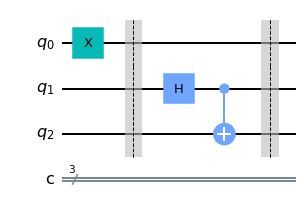
\includegraphics[width=0.5\linewidth]{Teleport3.png}
\caption{درهمتنیده‌شدن کیوبیت باب و آلیس}
\end{figure}
\end{center}

حال کیوبیت تلپورت و کیوبیت آلیس را درهم‌تنیده می‌کنیم:
\begin{tcolorbox}[width=13cm, colback=gray9, boxsep=10pt, halign=center]
\begin{Verbatim}[commandchars=\\\{\}]
\PY{n}{circuit}\PY{o}{.}\PY{n}{cx}\PY{p}{(}\PY{l+m+mi}{0}\PY{p}{,}\PY{l+m+mi}{1}\PY{p}{)}
\PY{n}{circuit}\PY{o}{.}\PY{n}{h}\PY{p}{(}\PY{l+m+mi}{0}\PY{p}{)}
\PY{n}{circuit}\PY{o}{.}\PY{n}{barrier}\PY{p}{(}\PY{p}{)}
\PY{n}{circuit}\PY{o}{.}\PY{n}{draw}\PY{p}{(}\PY{n}{output}\PY{o}{=}\PY{l+s+s1}{\PYZsq{}}\PY{l+s+s1}{mpl}\PY{l+s+s1}{\PYZsq{}}\PY{p}{)}
\end{Verbatim}
\end{tcolorbox}

\begin{center}
\begin{figure}[h]
\centering
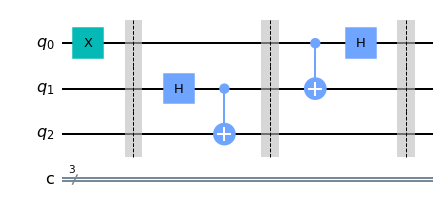
\includegraphics[width=0.8\linewidth]{Teleport4.png}
\caption{درهمتنیده‌شدن کیوبیت آلیس و کیولیت تلپورت}
\end{figure}
\end{center}

حال کیوبیت های صفر و یک (کیوبیت تلپورت و کیوبیت آلیس) را اندازه‌گیری می‌کنیم؛ سپس نتیجه را در بیت کلاسیک صفر و یک می‌گذاریم:
\begin{tcolorbox}[width=13cm, colback=gray9, boxsep=10pt, halign=center]
\begin{Verbatim}[commandchars=\\\{\}]
\PY{n}{circuit}\PY{o}{.}\PY{n}{measure}\PY{p}{(}\PY{p}{[}\PY{l+m+mi}{0}\PY{p}{,} \PY{l+m+mi}{1}\PY{p}{]}\PY{p}{,} \PY{p}{[}\PY{l+m+mi}{0}\PY{p}{,} \PY{l+m+mi}{1}\PY{p}{]}\PY{p}{)}
\PY{n}{circuit}\PY{o}{.}\PY{n}{barrier}\PY{p}{(}\PY{p}{)}
\PY{n}{circuit}\PY{o}{.}\PY{n}{draw}\PY{p}{(}\PY{n}{output}\PY{o}{=}\PY{l+s+s1}{\PYZsq{}}\PY{l+s+s1}{mpl}\PY{l+s+s1}{\PYZsq{}}\PY{p}{)}
\end{Verbatim}
\end{tcolorbox}
نتیجه‌ی نهایی به شکل زیر است:
\begin{center}
\begin{figure}[h]
\centering
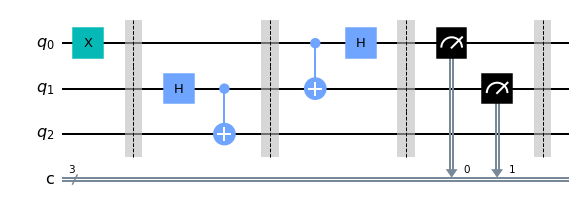
\includegraphics[width=0.8\linewidth]{Teleport5.png}
\caption{اندازه‌گیری کیوبیت آلیس و سای}
\end{figure}
\end{center}
باب با توجه به بیت‌های کلاسیکی که از سمت آلیس دریافت کرده،‌ باید یک سری گیت کوانتومی را به کیوبیت خود اعمال کند.

\begin{tcolorbox}[width=13cm, colback=gray9, boxsep=10pt, halign=center]
\begin{Verbatim}[commandchars=\\\{\}]
\PY{n}{circuit}\PY{o}{.}\PY{n}{cx}\PY{p}{(}\PY{l+m+mi}{1}\PY{p}{,} \PY{l+m+mi}{2}\PY{p}{)}
\PY{n}{circuit}\PY{o}{.}\PY{n}{cz}\PY{p}{(}\PY{l+m+mi}{0}\PY{p}{,} \PY{l+m+mi}{2}\PY{p}{)}
\PY{n}{circuit}\PY{o}{.}\PY{n}{measure}\PY{p}{(}\PY{p}{[}\PY{l+m+mi}{2}\PY{p}{]}\PY{p}{,} \PY{p}{[}\PY{l+m+mi}{2}\PY{p}{]}\PY{p}{)}
\PY{n}{circuit}\PY{o}{.}\PY{n}{draw}\PY{p}{(}\PY{n}{output}\PY{o}{=}\PY{l+s+s1}{\PYZsq{}}\PY{l+s+s1}{mpl}\PY{l+s+s1}{\PYZsq{}}\PY{p}{)}
\end{Verbatim}
\end{tcolorbox}

\begin{center}
\begin{figure}[h]
\centering
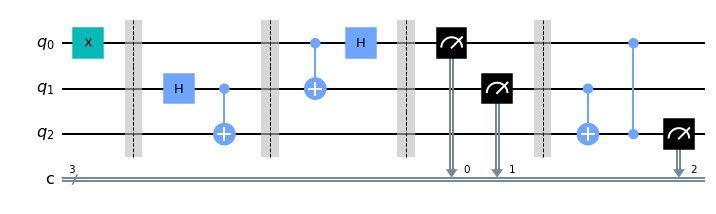
\includegraphics[width=1.1\linewidth]{Teleport6.png}
\caption{مرحله‌ی پایانی تلپورت، داده‌ی داخل کیوبیت سای به کیوبیت باب منتقل شده است.}
\end{figure}
\end{center}


حال مدار ایجاد شده را روی مدار پیاده سازی می‌کنیم:
\begin{tcolorbox}[width=13cm, colback=gray9, boxsep=10pt, halign=center]	
\begin{Verbatim}[commandchars=\\\{\}]
\PY{n}{simulator} \PY{o}{=} \PY{n}{Aer}\PY{o}{.}\PY{n}{get\PYZus{}backend}\PY{p}{(}\PY{l+s+s1}{\PYZsq{}}\PY{l+s+s1}{qasm\PYZus{}simulator}\PY{l+s+s1}{\PYZsq{}}\PY{p}{)}
\PY{n}{result} \PY{o}{=} \PY{n}{execute}\PY{p}{(}\PY{n}{circuit}\PY{p}{,} \PY{n}{backend}\PY{o}{=}\PY{n}{simulator}\PY{p}{,} \PY{n}{shots}\PY{o}{=}\PY{l+m+mi}{1024}\PY{p}{)}\PY{o}{.}\PY{n}{result}\PY{p}{(}\PY{p}{)}
\PY{k+kn}{from} \PY{n+nn}{qiskit}\PY{n+nn}{.}\PY{n+nn}{visualization} \PY{k+kn}{import} \PY{n}{plot\PYZus{}histogram}
\PY{n}{plot\PYZus{}histogram}\PY{p}{(}\PY{n}{result}\PY{o}{.}\PY{n}{get\PYZus{}counts}\PY{p}{(}\PY{n}{circuit}\PY{p}{)}\PY{p}{)}
\end{Verbatim}
\end{tcolorbox}

\begin{center}
\begin{figure}[h]
\centering
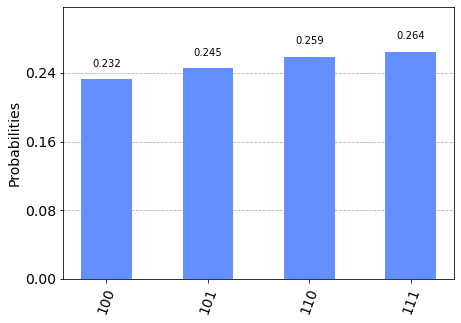
\includegraphics[width=0.8\linewidth]{Teleport7.png}
\caption{احتمال رخداد حالاتی که در آن مقدار کیوبیت تلپورت برابر یک است.}
\end{figure}
\end{center}

\textbf{از استاد بپرس چحوری ما حق داریم گیت ایکس و z را اثر بدهیم. چرا؟}
عدد اول بیانگر حالت کیوبیت اول است. تمامی حالاتی که مقدار این کیوبیت برابر یک باشد برای ما اهمیت دارد.

\end{document}